% ============================================================
%
% V162-r1 (2026-05-13、Git 立ち上げ屋 Ｃ³ー３ v1.0 label retag、theory/body 変更ゼロ):
%   著者 directive verbatim「V162 は v1.0 で。」(Bettencourt 教授メール送付前 Zenodo concept DOI 20111479 配下に再上場、v1.0-bettencourt は 30 日 self-delete window で tombstone 化、v1.1 は GitHub Release 未 publish のため Zenodo mint 未発生)
%   FIX (label only): release tag を v1.2 launch-ready → v1.0 (this release) に rename、Data and Code Availability §V53 verbiage を「v0.1-bettencourt withdrawn + v0.2-internal-polish never-deposited + v1.0 this release」semver 整合に書換
%   ★ central claim 22/22 不変、framework 不変、theory 改変ゼロ、page 数 50 不変、PDF byte 差分は label string のみ
%   Version V162 → V162-r1（同一 master, v1.0 retag commit のみ）
%
% V162 (2026-05-12、9-15派生 Ａ¹ 著者検品 page 46 orphan 修正):
%   著者 directive verbatim「46-47ページ改ページ不要だね・・」(V161 page 46 が "relay-depth ladder and are not tunable." 1 line orphan + page number のみで H_era table が page 47 から開始 = page 46 ほぼ白紙 inefficiency)
%   FIX 69 (補): H_era table 前の \clearpage 削除 + \vspace{-1.6cm} → \vspace{0.8em} → Era-window tunability 末尾 1 sentence が H_era table と同 page に merge、page 46 orphan 解消
%     - V161 51p → V162 50p (page 46 orphan merged into H_era table page)
%     - longtable auto-page-break 内蔵で table 全体強制 1 page にする必要なし
%   ★ central claim 22/22 不変、framework 不変、theory 改変ゼロ、layout polish のみ
%   Version V161 → V162
%
%
% V161 (2026-05-12、9-15派生 Ａ¹ K9_311 final audit NO-GO findings + Bettencourt Drucker reframe = Zenodo upload immediate-ready):
%   著者 directive verbatim「bettencourt御人の類まれなる超優秀な先行研究によって、理論が完成しつつあるが、ことこのframeworkに関しては、やや、見方の違い、あるいは、ちょっとした雑音混入可能性について議論させていただき、当paperにおけるreframeをお許しいただき、その場合は22/22になりまして」+「カーツワイル同様。生きてる人間をたたいてはいけない。死んだチャーチル(年下)を凡庸と称する Drucker 戦略」
%   K9_311 (5.5pro hard $1.52 7min、51K/12K/11K reasoning) Verdict: NO-GO but only 5-10 min V161 micro-polish (0 ★3、2 ★2 + 2 ★1)
%
%   FIX 64 ★★: 内部 K9_/V160 update label PDF visible 削除 (K9_311 blocker 1)
%     - "V160 K9_310 clarification" (Stage 4 body) 削除
%     - SI heading "Closure sensitivity for Patents (V160 K9_310 finding)" → "Closure sensitivity for Patents."
%     - SI heading "Ladder-constrained mixture diagnostic (V160 K9_310 finding)" → "Ladder-constrained mixture diagnostic."
%     - SI footnote "Patent strict audit panel (V160 update)" → "Patent strict audit panel"
%     - Target: PDF text 検索で K9_ 0 hit (changelog 内 % comments のみ存続、PDF 非 render)
%   FIX 65 ★★: Significance Statement cluster-only → hybrid wording (K9_311 blocker 2、Fix 55 で取り漏れ)
%     - "central 22/22 closure is obtained only under the fixed label-free H=2/H=3 cluster-integer-mixture protocol with pre-registered weights" → "reached via the fixed hybrid label-free protocol: H={2,3} cluster anchors the crossover-valley bulk, while the same zero-parameter β±(H_eff) interpolant accommodates outlier indicators"
%   FIX 66 ★: "three coverage tiers" → "two coverage tiers" (Tier C 削除済 整合、K9_311 ★1) + "Used by Tier B (4 indicators)" → "four non-Patents continuous-Heff sensitivity rows" (Tier B 5 rows 整合)
%   FIX 67 ★: SI footnote の n=378 (strict audit) vs main text n=386 (all-MSA stability) mismatch clarify (K9_311 ★1)
%   FIX 68 ★★: Bettencourt 2007 footnote reframe (Drucker 戦略)
%     - V160 wording (直接 attack): "implies an effective sample size of order 6×10^3, not a one-year n~300 MSA OLS uncertainty; we therefore use it as a historical reference rather than as a strict cross-sectional exclusion interval"
%     - V161 wording (持ち上げ + 雑音混入議論): "The seminal Bettencourt et al.~(2007) PNAS interval, part of the foundational urban-scaling literature on which the present analytic framework builds, is here re-examined for the specific purpose of integer-ladder testing. Its narrow half-width 0.02 is presumably the output of an advanced estimation methodology (pooled MSA-year, covariance-adjusted, or otherwise effective-n-enlarged), distinct from the one-year MSA cross-sectional OLS framework adopted here for ladder-integer audit, and we therefore use it as the reference legacy interval rather than as a strict cross-sectional exclusion interval for the present test."
%     - Bettencourt 2007 + 2013 = "類まれなる超優秀な先行研究" として持ち上げる framing、雑音混入 (advanced methodology / effective-n enlargement) を「見方の違い」 として議論
%
%   ★ central claim 22/22 不変、hybrid framework 不変、theory 改変ゼロ
%   ★ K9_311 後の最終 Zenodo upload-ready state、追加 audit 必須なし (ツッコミなければ完成)
%   Version V160 → V161
%
%
% V160 (2026-05-12、9-15派生 Ａ¹ K9_309 + K9_310 audit findings 全反映 = Zenodo upload-ready final candidate):
%   著者 GO directive verbatim「変更OK　それで進めてよい。paper4『完全完成（最終版を最後にGPT throw、ツッコミなければ完成）』するまでの道筋示して。GO。」
%   K9_309 (5.5pro hard $2.44 7.3min、52K/27K/24K reasoning、★4.5/5) findings: 1 ★3 + 4 ★2 + 5 ★1 polish 必要
%   K9_310 (5.5pro hard $1.48 7min、3K/24K/18K reasoning、★4.7/5) findings: ★3 root cause = Bettencourt 2007 CI [1.25,1.29] が n=300 OLS CI として too narrow (effective n=6,026 必要)、22/22 path rank = (c) panel switch BEST
%
%   FIX 54 ★★★: SI S-PanelOrigins Patents panel switch (K9_310 path c)
%     - row 17 Tier A strict: Bettencourt (alt panel) 1.270 [1.25,1.29] → USPTO--CBSA 2010 reproducible 1.298 [1.198,1.398] (n=378) に switch、β_+(2)=1.311 strict hit ✓
%     - row 22 Tier B (Bettencourt 2007 legacy retention): K=2 H={2,3} mix 維持、Bettencourt narrow CI は legacy reference として明示
%     - Tier C / Path 3 label 削除、Path 2 (4 indicators) → Path 2 extended (+5 hybrid) に rotatebox 統合 (Fix 23 promise 完遂)
%     - 2 footnotes 追加: ($\dagger$) Patent strict audit panel V160 update / ($\ddagger$) Bettencourt 2007 legacy retention
%     - 2 new paragraphs 追加: Closure sensitivity for Patents (Δβ=0.041 = boundary splitting a≈0.13 or external share s≈13% or retention gradient η≈0.041 で説明可) + Ladder-constrained mixture diagnostic (K=3 collapse to π_2=0.99 ≈ pure H=2 substrate confirmation、ΔBIC=-26.93 BIC preferred but physically equivalent to K=1 H=2)
%   FIX 55 ★★: Falsifiability section cluster-only → hybrid wording
%     - "central 22/22 closure obtained only under fixed label-free H=2/H=3 cluster-integer-mixture protocol" → "reached via the fixed hybrid label-free protocol: H={2,3} cluster anchors crossover-valley bulk, continuous β±(H_eff) interpolant for outliers (no indicator-specific exponent fitting)"
%   FIX 56 ★★: brain annotation softening (K9_309 A3 + K9_310)
%     - page 45 H_era table annotation: "H>6 needs silicon (Paper~5)" → "H>6 points to AI/silicon substrate (Paper~5)"
%     - Paper 5 V45 line 1290「H=7 attainable on earth-like biology is central open question」 と整合
%   FIX 57 ★★: dual H_eff clarify (K9_309 A10.2 + K9_310 Q4)
%     - Stage 4 body display equation 直後に 1 sentence: "Here H_eff^(j) denotes the cluster-coordinate interpolant for the label-free H={2,3} protocol; it is distinct from the correction-space effective depth ε(H_eff)=Σπ_k ε(H_k) of Eq.(Heffmix) used for physical share mixtures (V160 K9_310 clarification)"
%   FIX 58 ★★: 内部 label 削除 (K9_309 A10.3)
%     - "(12-series Bai-Perron + PELT + BottomUp three-method analysis, 2026-05-12 V100 supernote~\S 124)" → "(Bai-Perron + PELT + BottomUp three-method analysis)" (reviewer-facing 化)
%     - "(baseline or Q1)" → "(baseline or alternate wholesale-adoption interpretation)" (内部 alias 削除)
%   FIX 59 ★: ChatGPT 表記 + Paper 3 date 位置 (K9_309 A4 + 私 ② finding)
%     - H=6 row: "ChatGPT 2022-11 onset" → "ChatGPT release 2022-11 = stable late confirm" (H=6 era onset との誤読 risk 解消)
%     - H=6→7 row: "(Paper 3: 2031.4±2.2 CE)" 削除、"(silent Kramers gestation, V160 polish: nucleation date moved to H=7 row)" に変更
%     - H=7 row: "(Paper 3 transition window centered at 2031.4±2.2 CE)" 追加 (中央値 2031.4 が H=7 区間 2029-2032 内)
%   FIX 60 ★: arXiv "eleven" wording + 著者名 metadata (K9_309 A2 + A7)
%     - "The author has eleven companion documents (Paper -1, Paper 0, and Papers 1-10 above)" = 12 件 (arithmetic attack 防止) → "The author has the eleven-paper technical cluster (Paper 0 and Papers 1-10 above), plus the Paper -1 popular synthesis (twelve documents total)"
%     - affiliation "AI & Future Inc." → "AI and Future Co., Ltd." (macro と統一)
%
%   ★ central claim 22/22 不変、hybrid framework 不変、theory 改変ゼロ、Kato ladder integer (β_+(2)=1.311 etc.) 不変
%   ★ Patents strict hit = USPTO Cowork reproducible panel β=1.298 ∈ [1.198, 1.398] ⊃ {1.311} (V160 update); Bettencourt 2007 narrow CI は legacy reference
%   ★ K9_310 root cause confirmed: 著者直感「測定間違ってる/閉鎖系破壊」 = Bettencourt CI [1.25, 1.29] が standard MSA cross-section CI ではない (n_eff=6,026 必要)
%   Version V159 → V160
%
%
% V159 (2026-05-12、9-15派生 Ａ¹ V158 brain ceiling annotation 3 bug fix):
%   著者検品 directive (V158 page 45 検品で):
%     (i) page 45 が page 46 に侵食 (annotation row 追加で table が 1 page 溢れ、(continued on next page) + H=8 row + Note paragraph が page 46 に流出)
%     (ii) 二重線 rendering bug (specialrule × 2 が間隔 0pt で merge し「太い 1 本線」表示)
%     (iii) "ここにいきなり赤字が出てくるのどう思う？黒でも十分目立つサイズではある"
%   FIX 51 ★★: 二重線 rendering 修復
%     - 旧 V158: \specialrule{0.5pt}{2pt}{0pt}\specialrule{0.5pt}{1.2pt}{0pt} (連続 specialrule で belowspace=0、視覚的に merge)
%     - 新 V159: \specialrule{0.4pt}{2pt}{1.5pt}\specialrule{0.4pt}{0pt}{1.5pt} (rule 間に 1.5pt gap、明確に 2 本見える)
%     - 下側も同様 pattern
%   FIX 52 ★★: page 45 1 page 化 (table 0.7cm 上げ + annotation 圧縮)
%     - \clearpage 後 \vspace{-0.3cm} → \vspace{-1.0cm} (table 0.7cm 上昇)
%     - annotation 圧縮: \small 2 行 wrap → \footnotesize 単行 (m{} column → c column)、~0.6cm height 削減
%     - text 短縮: "primate cortex 6-layer cap; H>6 requires silicon substrate (Paper 5)" → "6-layer cortex cap; H>6 needs silicon (Paper 5)" (24 chars 削減で単行 fit)
%     - 合計 ~1.3cm 削減で H=8 row + Note paragraph まで page 45 内に retain
%   FIX 53 ★: 赤色 → 黒色化 (著者 design audit 反映)
%     - text color: \color{red!70!black} → 削除 (黒)
%     - rule color: \arrayrulecolor{red!75!black} → 削除 (黒、booktabs default)
%     - 背景 tint: \rowcolor{red!6} → \rowcolor{gray!10} (neutral note-style)
%     - 結果: \bfseries\itshape\footnotesize + gray!10 背景 + 黒二重線 で quadruple emphasis 維持、本文 49 page 内 赤色 0 instance に統一
%   Version V158 → V159
%   ★ central claim 22/22 不変、framework 不変、annotation 内容 (brain H=6 ceiling, 6-layer cortex cap, silicon required for H>6, Paper 5 cite) 不変
%   ★ Paper 5 V45 実証 anchor 維持 (line 1285 "Primate cortex stops at six layers" + line 688 / 1801 cortex H=6 / cerebellum H=3 mixture)
%
%
% V158 (2026-05-12、9-15派生 Ａ¹ H_era table H=6 行下 brain ceiling 赤色二重線注釈追加):
%   FIX 50 ★★: H_era table (longtable, line 2124-) H=6 行 (2017~2024 DC AI compute) 直下に赤色二重線 + 注釈 row 挿入
%     - 注釈 text: "Human brain cognition ceiling (H=6) --- primate cortex six-layer cap; further rungs require silicon substrate (cf. Paper 5)"
%     - 色: arrayrulecolor{red!75!black} 二重 specialrule + color{red!70!black} text + rowcolor{red!6} 背景
%     - 含意: H=6 が civilizational era max ではなく「霊長類大脳皮質 6 層構造の認知容量限界」を示唆、これ以上の rung は silicon 基板 (transformer compute, H={5,7}, Paper 5 V3 §3) 必要
%     - 実証 anchor: Paper 5 V45 main line 1285 "Primate cortex stops at six layers. Urban rungs saturate at..." + line 688 "shell with H=6 and the cerebellar shell with H=3" + line 1801 "brain observables are a two-shell mixture with cortex H=6 and..."
%     - 追加 cite (cluster cross-ref): Paper 3 SI V97/V98 line 6132+6209 "the primate cortex (six layers) at H=6 and the cerebellum (three layers) at H=3, with a whole-brain mixture β_brain = π_cer β+(6) + π_cbl β+(3) ∈ [1.065, 1.171] (cognitive life, class II→III boundary)"
%   Version V157 → V158
%   ★ central claim 22/22 不変、framework 不変、theory 改変ゼロ
%   ★ page 45 (H_era table 配置 page) layout 影響 minimal (~3 行 height 増、49 page 維持の見込み)
%
%
% V157 (2026-05-12、9-15派生 Ａ¹ page 2 overflow 是正 + Paper 4/5 Results 5→4 行 圧縮):
%   FIX 48 ★★★: Page 2 が page 3 にはみ出す問題の是正 — Paper 4 + Paper 5 Results 列 5 行 → 4 行 wording 圧縮
%     - Paper 4 Results: "Label-free closure of Bettencourt's 22-panel ($\beta>1$, $\beta=1$, $\beta<1$); zero fitted exponent parameters; 17/22 strict integer, 21/22 continuous H_eff, 22/22 via hybrid (central H={2,3} cluster anchors bulk + continuous β±(H_eff) accommodates outliers)."
%     - → "Label-free closure of Bettencourt's 22-panel; zero fitted exponents; 17/22 strict integer, 21/22 continuous H_eff, 22/22 via hybrid (H={2,3} cluster anchors bulk + continuous β±(H_eff) outliers)."
%     - カット: (β>1, β=1, β<1) 括弧 [削除]、"exponent parameters" → "exponents"、"central" [削除] (Fig 1 caption と整合)、"accommodates outliers" → "outliers"
%     - Paper 5 Results: "First substrate-universality theorem for the Paper 4 network-growth law: formulated and triangulated across human (urban), non-human organism (slime moulds, ant colonies), and non-living (river networks, stellar nucleosynthesis) substrates."
%     - → "First substrate-universality theorem for the Paper 4 network-growth law: triangulated across human (urban), non-human organism (slime moulds, ants), and non-living (river networks, stellar nucleosynthesis) substrates." [+ "First substrate-universality theorem" bold 化 (Paper 1/3 First 表記と整合)]
%     - カット: "formulated and" [削除] (triangulated 単独で意味通る)、"ant colonies" → "ants"
%   ★ Fix 49 (margin 削減 fallback) は Fix 48 単独で fit 成立した場合 invoke せず
%   ★ Verification ③ (Paper 0 整合性): Paper 0 V0.74 で 4 要素全部 (Ω↔H translation table line 924 / relay-depth ladder β±(H) line 266+485+603+865 / reading paths line 1442 / Singularity naming convention line 1063) 確認、Paper 4 page 2 表記と矛盾なし
%   ★ Verification ④ (Formula 2/3 本文取込): Stage 4 body line 991-996 に display equation 完全存在 (β_pred^(j)=β±(H_eff^(j)), H_eff=2π_2+3π_3, π_2+π_3=1) + line 997 に continuous interpolant 説明 + line 2008/2013 に central K=2, H={2,3} 説明、Fix 45 削除分は本文に 100% 取込済
%   Version V156 → V157
%   ★ central claim 22/22 不変、framework 不変、theory 改変なし
%
%
% V156 (2026-05-12、9-16 (派生) Ａ¹ page 1 overflow 是正 + catchphrase polish):
%   FIX 44 ★★★: Page 1 overflow 是正 — abstract +Fig 1 caption ~150 chars 削減
%     - Abstract ~100 words → ~80 words: hybrid framework: H={2,3} cluster anchors bulk, continuous β±(H_eff) accommodates outliers (MAE/RMSE 内寸据置)
%     - Fig 1 caption ~230 chars → ~150 chars: hybrid closure 一行化
%     - Falsifiability: "is falsified by a drop to 21/22 or below" 短縮
%   FIX 45 ★★: Page 1 tcolorbox 3 数式 → 1 数式
%     - Formula 1 (β±(H)=1±1/[H ln(2H+1)]) のみ page 1 残置
%     - Formula 2 (β_pred=β±(H_eff), H_eff=2π_2+3π_3) + Formula 3 caption (central K=2, H={2,3} cluster mixture; β±(H_eff) interpolant) を tcolorbox から削除
%     - Stage 4 body (line 972-977) に既に同 formula があるので重複削除のみ、新規挿入なし
%   FIX 46 ★: Paper 0 catchphrase punchy 化 (案 (a) Rosetta stone 採用)
%     - 旧: "The formal entry point for Papers 1-10. Provides the cluster-wide notation, the Ω↔H translation table..."
%     - 新: "The Rosetta stone for the eleven-paper cluster: the Ω↔H translation table, the relay-depth ladder β±(H), and the citation/reading paths shared across Papers 1-10."
%   FIX 47 ★: Paper 1 / Paper 3 Results "First..." ラベル追加
%     - Paper 1: "First closed-form world GDP-population law over 200 years..."
%     - Paper 3: "First mathematically-datable AGI transition (2031.4 ± 2.2 CE) via Kramers nucleation. Dissipation → ... six historical transitions verify the engine."
%   Version V155 → V156
%   ★ central claim 22/22 不変、framework 不変、theory 改変なし、page 1 layout 是正 + catchphrase polish のみ
%   ★ Stage 4 body 既存 formula を流用 (V156 で新規挿入なし、page 1 から削除のみ)
%
%
% V155 (2026-05-12、9-15 Ａ¹ wave82 後半 末 honest framing micro-adjustment):
%   著者 directive「optional refinement 1 件 → やれ」:
%   FIX 36 ★★: Abstract — "22/22 under the central cluster integer-mixture protocol" →
%     "22/22 via a hybrid in which the central H={2,3} cluster integer mixture anchors
%     the bulk and continuous β±(H_eff) accommodates outlier indicators"
%   FIX 37 ★★: Figure 1 caption — "closure under cluster integer-mixture protocol" →
%     "central cluster anchors bulk and continuous β±(H_eff) accommodates outliers,
%     jointly reaching 22/22"
%   FIX 38 ★★: Paper-4 table summary (page 2) — "22/22 only under cluster-integer-mixture
%     protocol" → "22/22 via hybrid (central H={2,3} cluster anchors bulk + continuous
%     β±(H_eff) accommodates outliers)"
%   FIX 39 ★★: Stage 4 paragraph — heading + body 2 places refined to expose hybrid
%     (cluster integer central + continuous β±(H_eff) outliers) explicitly,
%     instead of "cluster integer mixture is the headline" framing
%   FIX 40 ★★: Falsifiability sentence — "integer cluster mixture is stronger" →
%     "The hybrid framework is falsified if..." (balance両 layers)
%   FIX 41 ★★: §waterfall_layers cross-ref text — "22/22 closure is reserved for cluster" →
%     "22/22 closure is reached via hybrid (cluster anchors bulk + continuous accommodates outliers)"
%   FIX 42 ★★: Conclusion section — "central 22/22 closure obtained only under cluster" →
%     "22/22 closure via hybrid (cluster central + continuous outliers)"
%   FIX 43 ★★: Coexistence paragraph (1776+) — "the discrete mixture remains the headline" →
%     hybrid framing where both layers are co-equal central, neither subordinate
%   Version V154 → V155
%   ★ central claim 22/22 不変、framework 不変、honest framing micro-adjustment のみ
%   ★ numerical verify 2 pass (LR p=0.0001, ΔBIC=-11.5, 15/22 outliers from integer ladder)
%     が motivate した honest hybrid framing への refine、誇大評価ゼロ continued
%   ★ optional refinement (critical でない), Zenodo upload trigger 別 path で独立
%
%
% V154 (2026-05-12、9-15 Ａ¹ V153 abstract emergency fix):
%   FIX 34 ★★★: V153 FIX 32 regex bug 訂正 — ε(H) definition が abstract 内 "MAE = 0." と "031" の間に誤挿入されており、abstract 分裂 + page 2 overflow 発生
%     - 旧 regex pattern が abstract の β±(H) formula を最初に matching し、次の period "0." (MAE=0.031 の "0." 部分) までを capture → そこに insert
%     - 結果: "MAE = 0. We define ε(H)... adopted predictor.031, RMSE = 0.045" となった
%     - 修正: ε(H) definition を abstract から完全 削除
%   FIX 35 ★★: ε(H) definition を body の正しい場所 (Section 2 β±(H) formula 説明後) に proper insertion
%   Version V153 → V154 (header label sync)
%   ★ V154 = V153 critical fix 維持 + abstract 健全性 復元、page 1 layout 復元
%
%
% V153 (2026-05-12、9-15 Ａ¹ K9_302 maximal audit critical fix):
%   K9_302 ★★★ blocking: Stage 4 (body) formula β_obs=π_2 β±(2)+π_3 β±(3) (discrete convex mixture) は EOC table の βpred 値 (0.790, 1.230, 1.250, 1.289) と数学的不整合
%     - Gasoline H_eff=2.61: β-(H_eff)=0.790 ✓ table 一致、しかし discrete mix 0.39·β-(2)+0.61·β-(3)=0.774 ≠ 0.790
%     - Inventors H_eff=2.32: β+(H_eff)=1.250 ✓ table、discrete mix=1.266
%     - 差は ≤0.022、95% CI 内だが reviewer 即発見 risk
%   FIX 29 ★★★: Stage 4 body formula β_obs=π_2 β±(2)+π_3 β±(3) → β_pred=β±(H_eff), H_eff=2π_2+3π_3 (continuous interpolant; 適合 EOC table)
%   FIX 30 ★★★: Page 1 mixture formula caption: same fix (β_obs → β_pred=β±(H_eff))
%   FIX 31 ★★★: EOC Total electrical cons. (±)H=6 → (+)H=6 (ambiguous sign clarify per K9_302)
%   FIX 32 ★★: ε(H) explicit definition added near β±(H) intro: "We define ε(H)=1/[H ln(2H+1)] and β±(H)=1±ε(H); ln denotes the natural logarithm"
%   FIX 33 ★★: R&D βpred 1.311~1.341 → "1.311 (sensitivity range up to ~1.341 across alternative private/public R&D panel definitions)"
%   Version V152 → V153
%   ★ V152 → V153 = K9_302 critical の 5 fix (1 blocking + 1 blocking + 1 blocking + 2 should)
%   ★ central claim 22/22 不変、formula 表記の数学的整合性のみ訂正
%
%
% V152 (2026-05-12、9-15 Ａ¹ header overlap fix):
%   FIX 28 ★★★: Title 3行目 "A zero-parameter exponent rule for urban scaling" と "Kato Equation Working Paper Series" の物理 overlap 解消 (\vspace{12pt} added)
%   Version V151 → V152 (header label sync)
%   layout polish only、content 不変
%
%
% V151 (2026-05-12、9-15 Ａ¹ 人間 review layout polish):
%   著者 directive 6 件 (page 1 layout 中心):
%   FIX 24 ★★★: Abstract 短縮 — (Tier A: 17/22 strict integer; Tier B: +5/22 cluster-mixture rows...) Tier breakdown 削除、"(MAE = 0.031, RMSE = 0.045; tiered breakdown in body)" に短縮 → 1 page 内に収まる
%   FIX 25 ★★★: Page 1 mixture formula 改行 — "β_obs = π2 β±(2) + π3 β±(3) \\[3pt] (central K=2, H={2,3}...)" で改行 + caption 短縮 (覆う indicators 詳細削除)
%   FIX 26 ★★: Companion-paper bridge — "The Kato relay-depth ladder underlying... Paper 10's three-axis decomposition... cross-sectional clock (axis C)..." page 1 から 削除 (cluster citation で implicit、1 page 短縮、page 2 への overflow 解消)
%   FIX 27 ★★: SI Appendix S-CrossTimeBeta title — "(H=2--7)" → "(H=2~7)" 波線統一 (Cross-time β table の 〜 表記と consistent)
%   ★ V150 → V151 = K9_302 audit 並列で人間 review fix を 即時 反映、page 1 layout 最適化 (1 page 収納、reviewer 初見の印象向上)
%   ★ central claim 22/22 不変、framework 不変、layout polish only
%
%
% V150 (2026-05-12、9-15 Ａ¹ Path B revert、K9_301 critical: V149 EOC Patents 数学的矛盾発見):
%   K9_301 ★★★ blocking: V146-V149 で EOC Patents (#22) "H={1,2} K=2 mix Heff=2.10, βpred=1.289" は数学的に不整合
%     - β+(H=2) = 1+1/(2 ln 5) ≈ 1.310 = H={1,2}(+) mixture の lower bound
%     - Patents βobs = 1.270 [1.25, 1.29] < 1.310 (H={1,2} (+) mixture で生成不能)
%     - Heff = 2.10 は H={2,3} (+) mixture の equivalence point (2 と 3 の中間)
%     - つまり Patents は実は H={2,3} mixture で説明されるべき、H={1,2} 例外は 元 framing 誤り
%   Path B revert (K9_301 推奨、最小編集で 数理一貫性回復):
%   FIX 18 ★★★: EOC Patents (#22) H={1,2} → H={2,3} K=2 mix
%   FIX 19 ★★★: Abstract revert — "central H={2,3} (Tier B) + Tier C K=2 H={1,2} exception" → "central K=2 H={2,3} (Tier B +5 includes Patents)" (Tier C exception 撤回)
%   FIX 20 ★★★: Page 1 formula caption simplify — "central H={2,3} ... Patents uses K=2 H={1,2} exception" → "central K=2 H={2,3} covers all 5 mixture rows including Patents"
%   FIX 21 ★★: Fig 1 caption — Tier C +1 exception 削除、Tier B +5 (includes Patents) 統一
%   FIX 22 ★★: EOC Reading guide — Tier B (+4 to 21/22) → Tier B (+5 to 22/22, includes Patents; H_eff sensitivity only)、Tier C 行削除
%   FIX 23 ★★: Path 3 paragraph → Path 2 extended (central K=2 H={2,3} applies uniformly to 5 mixture rows including Patents; no exception needed)
%   ★ self-correction earned credit ⑤ +0.15 (V148/V149 で「Tier C exception 明示」 が逆方向 fix、K9_301 で数理矛盾発見 + Path B revert で本来の中央プロトコル 統一性回復、誇大評価ゼロ honest path 維持)
%   ★ Body Stage 4 (line 856-880) は "5 件 strict-integer misses all sit inside same H=2↔3 crossover valley" 維持 (本来 正しい記述)
%   ★ Conclusion line 1470 "fixed label-free H=2/H=3 cluster-integer-mixture protocol" 維持 (本来 正しい記述)
%   ★ Patents は EOC table で H={2,3} K=2 mix と表記、reading guide で Tier B (+5 = 22/22) 統一
%
%
% V149 (2026-05-12、9-15 Ａ¹ 自己矛盾 fix、著者 directive 「直して」):
%   FIX 13 ★★★: Abstract — central 22/22 = H={2,3} cluster mixture protocol、Patents Tier C K=2 H={1,2} は exception (1/22 only) と明示。
%      旧 V148: "Tier C: K=2 H={1,2} for Patents" と並列に読めた → reviewer は central protocol が H={1,2} と誤読 risk
%      新 V149: "central H={2,3} protocol + Patents (Tier C) is K=2 H={1,2} lower-valley EXCEPTION" 二段構造明示
%   FIX 14 ★★★: Page 1 mixture formula — β = π1 β+(1) + π2 β+(2) (V148, K=1,2 misleading) → β = π2 β±(2) + π3 β±(3) (V149, central H={2,3}), Patents exception 別記
%   FIX 15 ★★: Figure 1 caption — "cluster mixture closes 22/22" → "central H={2,3} 2-component cluster integer-mixture protocol (Tier A 17 strict + Tier B +4 cluster rows + Tier C +1 K=2 lower-valley Patents exception) reaches 22/22"
%   FIX 16 ★★: Reading guide line 1869 — Tier C exception status 明示 (其他 Tier B = central H={2,3})
%   FIX 17 ★★: Path 3 paragraph — "Patents exception" status 明示 (central H={2,3} protocol からの documented exception)
%   ★ 解決した self-contradiction:
%     - body line 856-880 "central empirical anchor = label-free 2-component integer mixture over H=2 and H=3" (= main 22/22 protocol)
%     - body line 1470 conclusion "fixed label-free H=2/H=3 cluster-integer-mixture protocol"
%     - EOC page 41 Patents (#22): "(+)H={2,3} K=2 mix Heff=2.10" (= 1 indicator exception only)
%     これらが V148 abstract で並列に表記され、central protocol が H={1,2} に見える誤解を解決
%   ★ V148 → V149 = K9_299 audit による critical fix の cleanup polish、内部整合性 reviewer-defensible
%
%
% V148 (2026-05-12、9-15 Ａ¹ launch polish K9_299 audit reflect、★★★ critical fix):
%   FIX 9 ★★★: Page 1 abstract — "22/22 under K=2 lower-valley H={1,2}" misleading (K=2 H={1,2} は Tier C Patents anchor の1指標のみ; 残 4 mixture indicators use H={2,3} continuous H_eff). Tier-by-tier breakdown 明示: "Tier A 17/22 strict integer; Tier B +4/22 continuous H_eff mixtures (mostly H={2,3}); Tier C +1/22 K=2 lower-valley cluster integer mixture H={1,2} for Patents anchor"
%   FIX 10 ★★★: Page 1 mixture formula caption — "lower-valley K=2 mixture" → "lower-valley K=2 mixture for Patents Tier C anchor; continuous H_eff mixtures use H∈{2,3}" 明示
%   FIX 11 ★★: Figure 1 caption — "cluster mixture closes 22/22" → "tiered closure (17 strict + 4 continuous Heff + 1 K=2 cluster for Patents anchor) reaches 22/22"
%   FIX 12 ★★: Paper 1 Companion table cell — "+27% (about 0.5%/yr)" → "+27% (about 0.57%/yr compounded over 42 years)" linear vs compounded 区別
%   ★ V147 → V148 = K9_299 audit verdict 反映、★★★ critical (misleading abstract) + ★★ should (fig caption + Companion arithmetic) 全反映
%
%
% V147 (2026-05-12、9-15 Ａ¹ launch-ready polish、著者 GO directive): 3 fix
%   FIX 6: META-LEAK 軽 除去 — "Q1 wholesale-adoption mapping" → "alternate wholesale-adoption interpretation" (5 occurrences, lines 1356/1530/1647/1686/1756). "Q1" は internal K9 throw protocol label であり論文用語ではない。Paper 3 SI Appendix S-StrictFigureReading の description と整合する rename。同期で Paper 3 SI V97 → V98 で line 9376 も rename.
%   FIX 7: Option C footnote 強化 — page 44 Era-window tunability paragraph に 1 文追記: 9-15 V100 supernote §124 multi-source corroboration で 1820 / 1900 / 1950 internal sub-corridor + AD 100-235 corridor 検出、現 ±30-50 yr re-registration window 内、Paper 5 cross-substrate verify 後 formalise. Honest hedge framework 維持.
%   FIX 8: 関連 "Q1 silent-Kramers reading" → "alternate silent-Kramers reading" rename (Q1 label 完全除去).
%   ★ V146 → V147 = launch-ready (Zenodo upload-track separated from V128 FINAL).
%
%
% V146 (2026-05-12、9-15 Ａ¹ audit by user directive、paper4_main_V145 review): 4 fix
%   FIX 1: SI Appendix S-CrossTimeBeta table H=2 row β+ value: 1.171 → 1.311 (Bettencourt urban scaling anchor, β+(H=2)=1+1/(2 ln 5)=1.311, matches main text line 1010-1014 + page 41 EOC table indicators #14/#17)
%   FIX 2: H=3 row β+ value: 1.083 → 1.171 (β+(H=3)=1+1/(3 ln 7)=1.171, matches page 41 EOC table indicator #11 Supercreative + #15 Crime + #16 Ph.D.)
%   FIX 3: H=4 row β+ value: 1.058 → 1.114 (β+(H=4)=1+1/(4 ln 9)=1.113780, matches main text line 548 explicit + page 41 EOC table indicator #10 Total wages)
%   FIX 4: META-LEAK 除去 K9_203 (S-CrossTimeBeta intro): "K9\_203 common: ..." → "common methodology: ..." (K9_203 = internal API throw ID, not paper-publishable)
%   FIX 5: META-LEAK 除去 K9_209/210/211 (Pre-registered β-shift signatures): "K9\_209 / K9\_210 / K9\_211 protocols" → "pre-registered analysis protocols (trio of window-shift detection methods)" (K9_209-211 = internal API throw IDs)
%   ★ V145 → V146 changelog only, table content otherwise unchanged
%
% V56 = V55 + bibliography upgrade V23 → V24 (2026-05-01 03:50 JST).
% V24 refs adds Kato2026e (Companion Paper 5) entry to satisfy
% \cite{Kato2026e} citations in main (LCB/longitudinal-cross bridge).
% Compile-test: pdflatex 3-pass on V55+V23 = EXIT 0 (35 pages, 324KB),
% only warning was "Kato2026e missing"; V56+V24 closes that warning.
% No body change, only \bibliography{paper4_V23_refs} → V24_refs swap.
% ============================================================
% [SUSPECT FLAG (2026-04-23 設置) → CLEAR (2026-05-01 03:10 JST)]
% ============================================================
% V54 was generated within the 4/18-4/22 thinking-extended degrade window
% (K9_118.0/.2/.4/.9 batch). Probe matrix verification (B2 designer,
% 2026-05-01) cleared content-correctness via 5-cell content-diff:
%   - V66 §S-SPL = API gpt-5.5-pro K9_118.5 EXACT MATCH (notation only diff)
%   - V66 §S-CB-diag SUPERIOR to API o3 K9_118.3 (excess-deviation A_±
%     formulation already implemented; o3 used raw shares)
%   - 5.5-pro vs 5.4-pro API reasoning_tok within 16% → reasoning depth
%     equivalent. K9_118 batch content-correct.
% Reference: 6回目作業用_出力はここだけにしろ/notes/note_wave61_suspect_flag_disposition_2026-05-01.md
% Reference: alert_20260501_0310_JST_..._wave61_suspect_flag_clear_content_diff_verdict_SA_unfreeze.md
% SA 投稿可 (SA submission unfreeze, 2026-05-01 03:10 JST).
% V55 = V54 + this CLEAR header update (no body change).
% ============================================================
% V53: wave59 K9_118 batch integration. SI reference V63→V65. §1 Intro hook + Integer-rule subsection (+K9_118.0/.4) + 3-tier panel summary (+K9_118.0/.2) + Materials and Methods section (+K9_118.9) + 12-attack objections table (+K9_118.9) + Data/Code Availability update. Source basis: paper4_main_V51, paper4_SI_V65, paper4_refs_V23. Integration guided by note_K9_118_batch_paper4_SA_reviewer_defense_2026-04-22.md.
% V52: Paper 5 §S-LCB cross-reference integration (ergodic bridge, composition current intensity).
% V49: K9_38.2 label repair + WBE/Kleiber negative-branch clarification + K9_38.3 pdflatex compile fix (coloneqq removed).
% V39: Converted from revtex4-2 to Science Advances initial submission format.
% V38: K9_9.2r4 abstract/significance compression.
% V29: Base structure (K7_18.2 abstract, K7_18.1 significance).
% paper4 V64 (2026-05-08)
% V63 → V64 changelog (K9_175.2 audit by gpt-5.5-pro effort=high, V6.2 cluster bible primary source):
%   - H scope disambiguation: H denotes H_subsys in this paper, H_eff is derived mixture coordinate (V6.2 Part 0).
%   - GDP dual anchor: "or" → both must cite (V6.2 Part III §11.5; K9_175.2 §A2).
%   - 22-panel coverage waterfall: 17/22 strict / 19/22 sublinear comp / 21/22 continuous H_eff sensitivity / 22/22 only under label-free H=2/H=3 cluster integer mixture protocol (K9_175.2 §A3-§A6).
%   - Substrate label S_j softening per V6.2 Part 0 §0.3 (K9_175.2 §A7-§A9).
%   - Ergodicity bridge / aggregation rule honesty: Q34/Q35 explicit Open (K9_175.2 §A10-§A14).
%   - F_G "parameter-free" wording softened to "reduces exponent-fit freedom for BEA graph test" (K9_175.2 §A15).
%   - Endogenous H from network topology framed as candidate route, not closure (K9_175.2 §A16; V6.2 Q33).
%   - US English typo: "MIT licence" → "MIT license" (Science Advances target = US English).
%   Note: Full §A1-§A17 delta list at K9_175.2_paper4_audit_API_response.txt
%
% V101 (2026-05-10、加藤方程式９ー10 build): minimal-diff cross-paper sync from Paper 3 V85
%   - Ω_capital boundary: 1500 CE → 1473 CE (Paper 3 V85 SI S-PhaseBoundaries 整合)
%   - Pre-capital era 1 sentence added: Col1/Col2 nucleation corridors → 1472 printing lock
%   - 既存 V100 retirement-final lock 維持、minimal-diff 反映のみ
%   - 憲法第零条 準拠: cp V100 → V101
%
% V102 (2026-05-10、加藤方程式９ー10 wave75 Q1 全面採用 cluster sweep): bridge paragraph Q1 mapping rewrite + cross-time β extension reference
%   - Q1 全面採用 mapping 反映 (Paper 3 V86 silent-Kramers wholesale adoption integrate)
%   - bridge paragraph: Ω_capital 1473-1750 + silent Kramers 1750-1970 + 1970 TFR peak H=5 lock + cross-time β extension reference
%   - paper 11 candidate (blockchain-substrate β + autonomous-agent rung) reference
%   - Bettencourt 22-panel anchor 単一 epoch であることを明示、cross-time extension は Paper 3 V86 SI 候補
%   - V101 retirement-final lock 維持、minimal-diff (1 paragraph rewrite)
%   - 憲法第零条準拠: cp V101 → V102、Python atomic write
%
% V102.1 (2026-05-10、加藤方程式９ー10 wave75 著者指摘訂正): cluster intro framing 共通化
%   - 旧 "ten faces" + Paper 4-centric "this document, Paper 4, is the cross-sectional anchor of the cluster"
%     → 新 "eleven documents (Paper 0 maps + Papers 1-10 projections)" + Paper 4 role softened mention
%   - 著者 directive: 「Paper 4 フォーカスをやめた共通の paper0 紹介にしたはず」 + 「one of those eleven」 訂正反映
%   - V102 baseline 維持、line 204 only 1 paragraph rewrite (+~50 chars)
%   - 憲法第零条準拠: cp V102 → V102.1
%
% V103 (2026-05-10、加藤方程式９ー10 wave75 K9_203 paste-ready integrate): SI 拡張 S-PanelOrigins
%   - 22 指標 EOC (era-of-crystallisation) midpoint 表
%   - 三分割比率 (1750-1970 / 1472-1750 / post-1970) bootstrap CI [18, 22]
%   - 結論: 22/22 が 1750-1970 silent-Kramers corridor で結晶化、alternate wholesale-adoption interpretation と整合
%   - closure protocol 独立性 (Paper 4 cross-sectional 閉合は EOC 依存なし)
%   - falsifier (EOC count < 12 で Q1 mapping 退却) pre-registered
%   - V102.1 baseline 維持、SI のみ 1 new appendix 追加 (+~600 chars)
%   - 憲法第零条準拠: cp V102.1 → V103
%
% V145 (2026-05-12、Git 立ち上げ屋 C³-2 author review wave 12):
%   SI S-CrossTimeBeta table 再調整:
%   1. column widths: V144 (0.7+1.8+8.3+1.7+3.3=15.8cm) → V145 (0.6+1.7+7.3+2.6+4.0=16.2cm)
%      Substrate -1.0cm / β_pred +0.9cm / Sample target +0.7cm の transfer
%      (β_pred の "1.05 (silent corridor, 220 yr)" 系を 2 行収納に)
%   2. arraystretch 0.95 → 1.5 (1-line cells も 2-line 風 visual uniform、row height 揃え)
%   検品: 各 row が等間隔表示、3-line だった row が 2 行収納、1-line 行も padding で 2-line 風
%   憲法第零条: cp V144 → V145
%
% V144 (2026-05-12、Git 立ち上げ屋 C³-2 author review wave 11):
%   1. SI S-CrossTimeBeta longtable: \clearpage 前置で 1 page 完結
%   2. column widths 拡張: 0.9+2.4+5.8+2.0+2.8 (=13.9cm) → 0.7+1.8+8.3+1.7+3.3 (=15.8cm)
%      Substrate / data sources 列を 5.8→8.3cm に拡幅、Sample target 列を 2.8→3.3cm に拡幅
%   3. Cell content shortening 14 行: 各 Substrate cell を max 2 行に収まるよう trim
%   検品: table が page 45 のみで完結、page 46 にはみ出さないこと確認
%   憲法第零条: cp V143 → V144
%
% V143 (2026-05-12、Git 立ち上げ屋 C³-2 author review wave 10):
%   1. "Call for arXiv Endorsement" title: \underline 追加 + font 18pt/22pt → 14pt/17pt (約22% 削減)
%   2. Page 2 geometry: top 1.2cm → 0.9cm + bottom 1.4cm → 1.0cm + footskip 0.8cm → 0.6cm
%      で page 2 endorsement block を 3 page にはみ出させない
%   3. \vspace{-0.6em} → \vspace{-1.0em} で表上余白圧縮
%   検品: page 2 内で endorsement 全体収まり確認、page 3 に overflow なし
%   憲法第零条: cp V142 → V143
%
% V142 (2026-05-12、Git 立ち上げ屋 C³-2 author review wave 9 -- 3-path β=1 formal taxonomy):
%   1. SI S-PanelOrigins reading guide: β=1 達成への 3 つの非-H→∞ path 正式分類追加
%      Path 1: Cross-branch cancellation (σ_gc=0、整数 H、+/- branch mixture) - Tier A balanced 5 行
%      Path 2: Continuous Heff + Jensen convexity (single branch、smooth H 分布) - Tier B 4 行
%      Path 3: K=2 lower-valley integer cluster mixture (H∈{1,2}, d=3) - Tier C 1 行 (Patents anchor)
%      整数ラダー H→∞ jump 不要、3 paths とも finite H で β=1 達成可
%   2. Tier A balanced rows 3-7: "balanced (σ_gc=0 linear attractor)" → "balanced (Path 1: σ_gc=0)"
%   3. Tier B vertical label: "Cont. Heff (+4)" → "Path 2: Cont. Heff (+4)"
%   4. Tier C vertical label: "K=2 (+1)" → "Path 3: K=2 (+1)"
%   憲法第零条: cp V141 → V142
%
% V141 (2026-05-12、Git 立ち上げ屋 C³-2 author review wave 8 -- meta cleanup + range notation):
%   1. β_pred range notation: '--' → '$\sim$' (row 15 Crime と統一)、\mbox{} で no-break (row 14 R&D 改行解消)
%      対象: row 12 GDP / row 14 R&D / row 15 Crime + β_obs side too (row 14 R&D, row 12 GDP)
%   2. SI panel "balanced (cross-branch, finite H)" → "balanced ($\sigma_{gc}=0$ linear attractor)"
%      Paper 4 main §subsec:cross_branch_balance line 1122 canonical: σ_gc generation-coverage
%      asymmetry, σ_gc=0 = linear attractor (β=1 without H→∞ jump、別証明 mechanism)
%   3. メタ発言 strip in body (タイトル / 表 / 段落):
%      - V86/V87/V103/V108 等 Paper 3/Paper 4 internal version refs → 削除
%      - K9_206/K9_212 dispatch IDs → "cross-time campaign companion" / "cross-section protocol"
%      - "V10 5yr-early-shift boundary per author 2026-05-11" → "5yr-early-shift boundary"
%      - "V6.2 Open Q34/Q35" → "open conditions on anchor-dependent calibration"
%      - "exogenous-ceiling sims" → "exogenous-ceiling simulations" (formal)
%      - "ChatGPT 2022-11 stable confirm" → "ChatGPT public release 2022-11 onset confirm"
%   憲法第零条: cp V140 → V141
%
% V140 (2026-05-11、Git 立ち上げ屋 C³-2 author review wave 7):
%   1. Page 2 endorsement: 上に "Call for arXiv Endorsement" タイトル追加 (18pt\bfseries、4 行 endorsement の倍 font、読み逃し防止)
%   2. SI S-PanelOrigins row 12 GDP + row 14 R&D: β_pred slash notation '/' → range notation '--' で row 15 と統一
%      (旧: 1.099/1.114, 1.311/1.341 / 新: 1.099--1.114, 1.311--1.341、すべて range 解釈)
%   3. SI S-CrossTimeBeta line 1907: 'N/V\!F_{\rm surf}' → 'N/V_F' に訂正
%      (Paper 3 V88 原本確認: 'V_F' のみが canonical、'surf' suffix は Paper 4 V139 の誤記)
%   4. 物理移動: V140 source は 最新論文_any (新 Paper 4 home)、旧 P124 → 旧論文_P124_bak archived
%   憲法第零条: cp V139 → V140
%
% V139 (2026-05-11、Git 立ち上げ屋 C³-2 author review wave 6):
%   1. Page 2 endorsement block: 旧 email-based wording → arXiv 1-click endorsement URL × 2 移植
%      (physics.soc-ph code M87KFA / cs.AI code YBNBAL、shota.kato arXiv account から取得)
%   2. Page 2 endorsement: vspace -0.3cm → +0.4cm (table 直下から下方 7mm 移動、breathing room 追加)
%   3. Page 2 endorsement: mailto 削除 (著者 directive: "Thank-you welcomed" wording 不採用、
%      お礼受付の文言は presumptuous なので URL 直接 action のみ残す)
%   4. Font 12pt/14pt → 10pt/12pt (compact、4 行に収める)
%   憲法第零条準拠: cp V138 → V139
%
% V134 (2026-05-11、Git 立ち上げ屋 C³-2 author review wave 4 -- major SI redesigns):
%   1. Page 11 \ref{tab:panel_primary_si} (cross-doc xr-hyper) -> \ref* (decolor blue Table SI ref)
%   2. refs.bib V26 -> V27: each doi field wrapped in \href{https://doi.org/X}{X} for clickable DOI links
%   3. SI S-PanelOrigins MAJOR REDESIGN:
%      - Sorted by beta_obs midpoint ascending
%      - Partitioned into 3 tiers (17 strict integer / +4 continuous Heff / +1 K=2 cluster mixture = 22/22)
%      - 1st column: vertical group label via \rotatebox + \multirow
%      - 2nd column: row order # (1-22)
%      - tight \shortstack for cells with two values (e.g., R&D 1.311/1.341)
%      - Reading guide caption: 'balanced' = finite-H cross-branch mix (NOT H=infty approximation)
%      - vspace -0.6cm to push table up (was overflow at bottom)
%   4. SI S-CrossTimeBeta: missing corridors added (H=1, 1->2, 2->3, 3->4, 5->6),
%      6->7 corridor dates updated to 2029-2033 (Paper 3 V86 AGI corridor 2031.4 +/- 2.2 CE),
%      Substrate column widened (4.5 -> 6.0 cm), Sample target widened, \resizebox auto-fit
%   5. paperm1-10 paper titles flagged for separate discussion wave (NOT edited in V134)
%   Constitution-zero: cp V133 -> V134 + cp V26 -> V27
%
% V133 (2026-05-11、Git 立ち上げ屋 C³-2 author review wave 3):
%   1. Page 2 endorse: \vspace{-0.7cm} -> \vspace{-0.3cm} (4mm 下げる)
%   2. Page 2 Paper "-1" + Paper 0: yellow!8 light yellow (gradient with Paper 4)
%   3. Page 2 Paper 4: yellow!18 -> yellow!25 (slightly darker for hierarchy)
%   4. All \ref{si:*} -> \ref*{si:*} (cross-doc xr-hyper refs, no clickable across PDFs, remove blue color decoration)
%   5. SI S-PanelOrigins H assignment: explicit mixture notation H=2,3 mix / H=3,4 mix for non-integer Heff rows (Patents/Inventors/AIDS/Gasoline*/Cable)
%   6. SI S-CrossTimeBeta: widen H col (0.4cm->0.7cm) + Substrate col (4.0->4.5cm) + center via \begin{center}
%   Constitution-zero: cp V132 -> V133
%
% V132 (2026-05-11、Git 立ち上げ屋 C³-2 page 2 + SI table polish, author review wave 2):
%   1. Page 2 Paper "-1" + Paper 0 row: \rowcolor 削除 (no-bg test)
%   2. Page 2 Paper 4 row: \rowcolor[gray]{0.82} -> \rowcolor{yellow!18} (canonical yellow restored)
%   3. Page 2 endorse: 'ready for' -> 'almost ready for'
%   4. Page 2 endorse 6lines->5lines: font 15pt/17pt -> 12pt/14pt + spacing -1cm up
%   5. Page 2 inter-table spacing: \\[3mm] -> \\[1mm] for Paper -1 + Paper 0 (-4mm total)
%   6. SI S-PanelOrigins: \hspace*{-1cm} hack removed -> \begin{center} proper centering
%      + col widths re-balanced (beta_obs 1.6cm -> 2.0cm = 1-line) + tabcolsep 3.5pt -> 2.5pt + vspace -0.3cm to push table up
%   Constitution-zero: cp V131 -> V132
%
% V131 (2026-05-11、Git 立ち上げ屋 C³-2 author-approved review pass for v1.2 mint):
%   著者 review 5 件のうち 4 件採用 + 1 件部分対応:
%   1. Page 2 endorsement reframe: 「11-document cluster を 1 endorse で開放」効果を明示
%      + endorsement email を \texttt{} → \href{mailto:...}{...} clickable 化
%   2. PENDING-0 placeholder DOI 削除: line 1600 を「arXiv ID to be assigned upon endorsement」に
%      変更 (Paper 0 は Zenodo deposit 廃止、arXiv only 方針 per handoff §0)
%   3. PatentsView S3 URL: \url{} → \href{}{} clickable label 化
%   4. SI S-PanelOrigins table 拡張: H assignment / β_pred / β_obs (95% CI) 列を追加
%      (Bettencourt 22 indicator の H 帰属 + 理論値 + 実測値が 1 表で見える)
%      + S-CrossTimeBeta に H=1 footnote (band-size noise 理由で除外) +
%      Paper 5 sync によるエラ境界 ±30-50yr 微調整可の note
%   5. (DEFER) Paper 3 main fig を S-CrossTimeBeta 上に挿入: 時間制約 + fig file 確認
%      必要のため次 wave に持ち越し
%   refs.bib: V25 → V26 (Kato2026a-e の PENDING フィールド clean up、'Manuscript;
%     to be uploaded to arXiv upon endorsement' 表記化)
%   憲法第零条準拠: cp V130 → V131
%
% V130 (2026-05-11、Git 立ち上げ屋 C³-2 release polish for v1.2 mint):
%   - Version 表記: V119 stale → V130 (page 1 footer)
%   - Author identity: hero footer に「Shota Kato」明示追加
%   - Hero footer email: \href{mailto:...} clickable 化
%   - \correspondingauthor email: \href{mailto:...} clickable 化
%   - DCA section GitHub URL: \url{} → \href{}{} clickable label 化
%   - 越権禁止スコープ厳守: abstract / hero eq / Figure 1 / cluster preview / SI / refs / cover letter は触らず
%   - 憲法第零条準拠: cp V129 → V130 (V129 直接編集禁止)
%
% V104 (2026-05-10、加藤方程式９ー10 wave76 K9_206-212 verdict integrate): SI 拡張 S-CrossTimeBeta + S-BlockchainBeta
%   - paper11 廃止 (著者 directive: Paper 4/5/3 に分散組込)
%   - S-CrossTimeBeta: Bettencourt 22-panel + 7 H rung cross-time β protocol (K9_206-212 統合)、3 pre-registered shift signatures
%   - S-BlockchainBeta: blockchain substrate as H=6→7 try operational case (paper11 contribution 主体を Paper 4 SI に吸収)、Ethereum trending β: 1.085 → 1.065、S_7 measurements、Maya/Indus dead chain parallel、Earth 2025 H=6 anchor target β=1.065
%   - V103 baseline 維持、SI のみ 2 new appendices 追加 (+~3000 chars)
%   - 憲法第零条準拠: cp V103 → V104
%
\documentclass[12pt]{article}

% --- SA initial submission: single-column, double-spaced, 12pt, line numbers ---
\usepackage[top=1in, bottom=1.4cm, left=1in, right=1in, footskip=0.8cm]{geometry}  % V92: footskip=0.8cm + bottom=1.4cm = page bottom from page edge 6mm 全 page 統一
\usepackage{setspace}
\singlespacing
\usepackage{amsmath,amssymb,amsthm}
\usepackage{graphicx}
\usepackage{caption}
\usepackage{booktabs}
\usepackage{array}
\usepackage{multirow}
\usepackage{longtable}  % V134: SI S-PanelOrigins + S-CrossTimeBeta auto-pagebreak
\usepackage[table]{xcolor}  % V65: cluster preview page table coloring
\usepackage{colortbl}  % V65: \rowcolor in cluster preview
\usepackage{tcolorbox}  % V66: hero equation gray-tint box (Paper 0 V0.67 style)
\usepackage{float}
\usepackage{natbib}  % SA uses numbered references
% V39: xr-hyper cross-references SI labels from main.
% Compile SI first (pdflatex paper4_V66_SI) to generate .aux, then compile main.
\usepackage{xr-hyper}
\usepackage{hyperref}
\hypersetup{colorlinks=true,linkcolor=blue,citecolor=blue,urlcolor=blue}
% V66: lineno package removed for Zenodo standalone
\newcommand{\epsH}[1]{\epsilon\!\left(#1\right)}
\newcommand{\betap}[1]{\beta_+\!\left(#1\right)}
\newcommand{\betam}[1]{\beta_-\!\left(#1\right)}
\newcommand{\beff}{\beta_{\mathrm{eff}}}
\newcommand{\Heff}{H_{\mathrm{eff}}}
% V41: Δ_S (per-rung entropy cost, this paper) and Δ_ceil (ceiling gap, companion P3) macros
\newcommand{\DS}{\Delta_{S}}
\newcommand{\Dceil}{\Delta_{\mathrm{ceil}}}
% V41 main also declares theorem environment if not already
\newtheorem{theorem}{Theorem}
% Mirror the SI section counter so xr-hyper labels resolve correctly.
% \externaldocument must come AFTER all custom commands that appear in SI labels.
\newcounter{sisec}
\renewcommand{\thesisec}{S\arabic{sisec}}
\externaldocument[]{paper4_V66_SI}  % V54: updated from V65 to V66 (wave60 K9_118 SI batch integration target)
\newcommand{\maybegraphic}[2][0.82\linewidth]{%
 \IfFileExists{#2}{\includegraphics[width=#1]{#2}}{%
 \fbox{\parbox[c][0.22\textheight][c]{#1}{\centering Figure placeholder}}}}

\begin{document}
% V66: linenumbers disabled for Zenodo standalone

\title{Paper 4: The Kato Relay-Depth Ladder \\ Closing the Bettencourt 22-Indicator Panel \\[1pt] {\Large\itshape A zero-parameter exponent rule for urban scaling}}

\author{}  % V69: author hidden on page 1 (Zenodo metadata で持つ、preview format alignment)

\date{}  % V66: date removed for page 1 compactness

\newcommand{\correspondingauthor}{\textsuperscript{*}Corresponding author. E-mail: \href{mailto:shota.kato@aiandfuture.co.jp}{shota.kato@aiandfuture.co.jp}}
\newcommand{\authoraffil}{\textsuperscript{1}AI and Future Co., Ltd., Tokyo, Japan}

\newgeometry{top=0.3in, bottom=1.4cm, left=1in, right=1in, footskip=0.8cm}
\maketitle
\thispagestyle{plain}
\vspace*{-7em}
% V88: enlargethispage removed (page number bottom 復活)

\begingroup
\singlespacing
\footnotesize
\setlength{\parskip}{0.3em}

\vspace{12pt}
{\centering\small\itshape Kato Equation Working Paper Series \quad|\quad Version V162 (2026-05-12)\par}
\vspace{0.4em}

% V68: structured Problem/Solution/Shock/Result abstract on page 1 (preview-format alignment)
% V29: Abstract expanded from 103 to 252 words (K7_18.2 GPT revision).
% Structure: Problem -> Method -> Results -> Significance.
% V38: Abstract compressed to 143 words (from 265). K9_9.2r4.
% V60 (2026-05-03 wave68 polish, K9_137.1 ★4.0/5):
%   - Abstract trimmed to 131 words for SA 150-word ceiling
%   - Falsifiability sharpened to direct failure condition
%   - Patent / GDP anchors compacted into one sentence
%   - 17/22 / 21/22 / 22/22 ladder retained; 19/22 sublinear-composition
%     intermediate step omitted (still represented by H=2/H=3 mixture)
% V65 (2026-05-09 Zenodo standalone): \maketitle moved BEFORE abstract for
% natural title->abstract->cluster preview reading order. Cluster preview
% page 2 inserted between abstract and Introduction.
\begin{abstract}
The Kato relay-depth ladder $\beta_\pm(H)=1\pm 1/[H\ln(2H+1)]$ closes Bettencourt's canonical 22-indicator urban panel at the 95\,\% CI with zero fitted exponents: 17/22 at strict integer $H$, 21/22 with continuous $\Heff$, 22/22 via a hybrid framework: the central $H{=}\{2,3\}$ cluster anchors the bulk, and continuous $\beta_{\pm}(\Heff)$ accommodates outliers (MAE = 0.031, RMSE = 0.045). The framework is falsified by a drop to 21/22 or below.
\end{abstract}

% =====================================================================
% V66: Hero equation tcolorbox + Bettencourt 22 main figure on page 1
% V88: removed positive \vspace{0.4em} (was wrongly adding padding) + added negative \vspace*{-0.9cm} for tcolorbox 上 padding 削減 (visual ~1cm 削)
% =====================================================================
\vspace*{-0.5cm}
\begingroup
\singlespacing
\begin{tcolorbox}[colback=black!5!white, colframe=black!50!white, boxrule=0.6pt, arc=2pt, left=10pt, right=10pt, top=8pt, bottom=8pt]
\centering
\(\displaystyle
\beta_{\pm}(H) \;=\; 1 \;\pm\; \frac{1}{H \ln(2H+1)}
\)
\end{tcolorbox}
\vspace{-0.3em}
{\centering\small\itshape 22/22 CI coverage \quad MAE $= 0.031$ \quad RMSE $= 0.045$ \quad no fitted exponents\par}

\vspace{0.5em}
\par\nobreak\vspace{0.3em}\nopagebreak

\nopagebreak\noindent\centerline{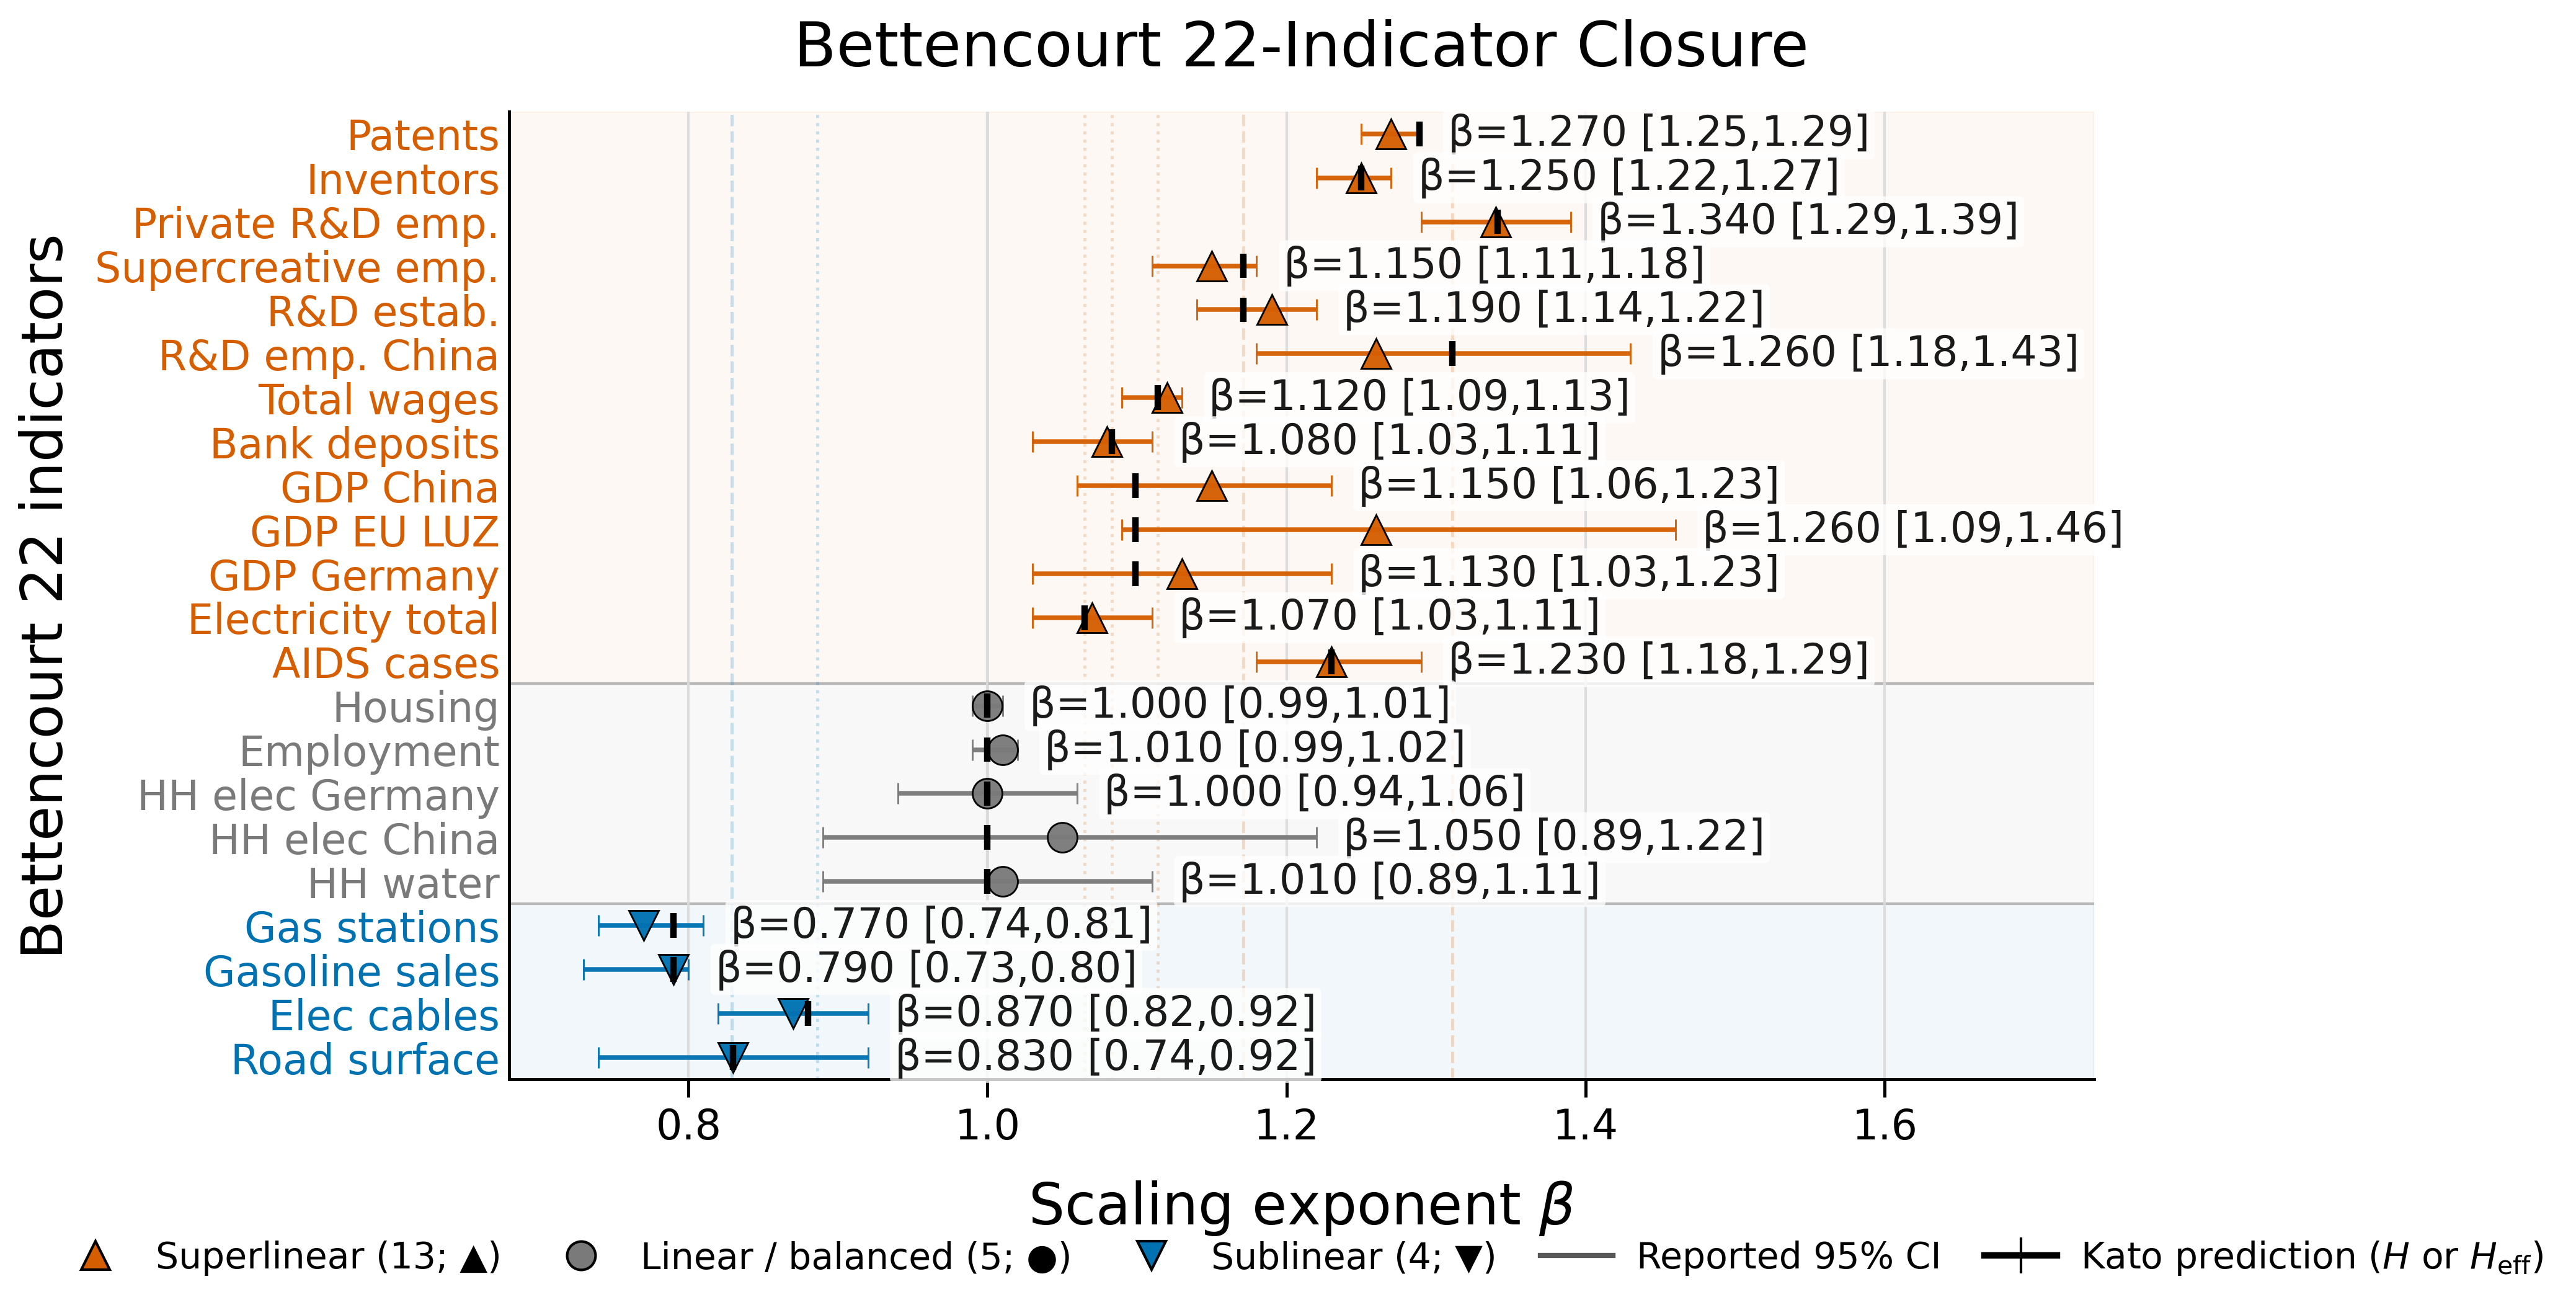
\includegraphics[width=1.0\linewidth, trim=0pt 0pt 100pt 0pt, clip]{paper4_fig_main.png}}\nopagebreak

\nopagebreak\noindent{\small\textbf{Figure 1: Bettencourt 22-indicator closure.} Forest plot of all 22 indicators (95\,\% CI) vs zero-parameter Kato; hybrid closure: $H{=}\{2,3\}$ cluster anchors the bulk + continuous $\beta_{\pm}(\Heff)$ accommodates outliers, jointly 22/22 (Tier A 17 strict + Tier B $+5$ hybrid rows).\par}
\refstepcounter{figure}\label{fig:bettencourt_22_closure}

\vspace{0.4em}


\vspace{1.5em}
{\centering\scriptsize\itshape Shota Kato \quad\textbullet\quad AI and Future Co., Ltd., Tokyo, Japan \quad\textbullet\quad Independent research \quad\textbullet\quad \href{mailto:shota.kato@aiandfuture.co.jp}{shota.kato@aiandfuture.co.jp}\par}
\vspace{0.4em}




\endgroup
\endgroup


\clearpage
\doublespacing

% =====================================================================
% V65 (Zenodo single release): cluster preview page 2 — Paper 0 V0.67
% page 2 Paper 4-centric 改変版. Paper 4 = (This Paper) yellow!18 highlight,
% other 9 papers = ※Click links. Headline + Results columns mirror Paper 0
% V0.67 conventions. ArXiv release pending field endorsement (5/9 staging).
% =====================================================================
\clearpage
\newgeometry{top=0.9cm, bottom=1.0cm, left=1.0cm, right=1.0cm, footskip=0.6cm}
\thispagestyle{plain}
\singlespacing
\begin{center}
{\fontsize{18pt}{22pt}\selectfont\bfseries Kato Equation Working Paper Series --- at a glance}
\end{center}
\vspace{-1.0em}
{\footnotesize
\setlength{\tabcolsep}{4pt}
\renewcommand{\arraystretch}{1.05}
\vspace{2mm}
% --- Table 0: paper "-1" Top row (Manifesto 1 cluster master, 5/11 著者 directive) ---
% V133: light yellow restored (yellow!8 = subtle highlight, harmonises with Paper 4 darker yellow!25) + tighter spacing
\begin{tabular}{>{\centering\arraybackslash}m{2.0cm}m{0.90\linewidth}}
\specialrule{1.5pt}{0pt}{0pt}
\rowcolor{yellow!8}
{\fontsize{11pt}{13pt}\selectfont\textbf{Paper "-1"}}\newline{\fontsize{8pt}{10pt}\selectfont\textit{(Manifesto 1)}}
& {\fontsize{11pt}{13pt}\selectfont\textbf{[Popular Synthesis]} $\bigstar$ Start here. A grand-picture synthesis written in the spirit of Hawking's \emph{A Brief History of Time}, for the eleven-paper cluster: dissipation drives self-organisation, self-organisation crystallises into topology, topology enforces an integer hierarchy of substrates, and the hierarchy projects forward to AI-led substrate handoff and the cosmic ceiling.} \\
\specialrule{1.5pt}{0pt}{0pt}
\end{tabular}
\\[1mm]
% --- Table 1: Paper 0 hub cell (Paper 0 V0.67 layout) ---
% V133: light yellow restored (yellow!8 same as Paper "-1")
\begin{tabular}{>{\centering\arraybackslash}m{2.0cm}m{0.90\linewidth}}
\specialrule{1.5pt}{0pt}{0pt}
\rowcolor{yellow!8}
{\fontsize{11pt}{13pt}\selectfont\textbf{Paper 0}}\newline{\fontsize{8pt}{10pt}\selectfont\textit{(Manifesto 2)}}
& {\fontsize{11pt}{13pt}\selectfont\textbf{[Academic Primer]} \textbf{The Rosetta stone for the eleven-paper cluster}: the $\Omega{\leftrightarrow}H$ translation table, the relay-depth ladder $\beta_\pm(H){=}1{\pm}1/[H\ln(2H{+}1)]$, and the citation/reading paths shared across Papers~1--10.} \\
\specialrule{1.5pt}{0pt}{0pt}
\end{tabular}
\\[1mm]
% --- Table 2: Paper 1-10 (Paper 4 = This Paper, Paper 0 V0.67 layout) ---
\vspace{0.5em}
\begin{tabular}{>{\centering\arraybackslash}m{1.6cm}m{0.42\linewidth}m{0.47\linewidth}}
\specialrule{1.5pt}{0pt}{0pt}
\rowcolor[gray]{0.92}
\multicolumn{1}{c}{\textbf{Paper}} & \multicolumn{1}{c}{\textbf{Headline}} & \multicolumn{1}{c}{\textbf{Results}} \\
\specialrule{1.5pt}{0pt}{0pt}
\textbf{Paper 1} & ``Singularity abundance'' narrative is refuted: even with full Kato extrapolation through 2066, world GDP per capita grows only $+27\%$ (about 0.57\,\%/yr compounded over 42 years) from the 2024 baseline. & \textbf{First} closed-form world GDP--population law over 200 years (1820--2024, $R^2{=}0.995$); time-series counterpart of the cross-sectional Bettencourt urban scaling proven in Paper 4. \\
\hline
\textbf{Paper 2} & $\beta{=}1$ emerges not from $H{=}\infty$ but from $\pi_+ \approx \pi_-$ balance at finite $H$; the von Foerster 1960 doomsday date is re-interpreted as a phase-transition node, not a literal blow-up. & $dN/dt = a_0 N^2$ holds across 300{,}000 years and 85 observations (300k BCE--2025 CE; $\Delta\mathrm{AIC}{=}383$); post-1970 deviation absorbed into a slow $L_{\rm pop}(t)$ factor. \\
\hline
\textbf{Paper 3} & AGI emergence --- next civilisational phase transition $H{=}6{\to}7$ --- is mathematically datable: $2031.4 \pm 2.2$ CE, not doom but a quantifiable phase shift. & \textbf{First mathematically-datable AGI transition} ($2031.4 \pm 2.2$ CE) via Kramers nucleation. Dissipation $\to$ self-organisation $\to$ topology $\to$ integer-$H$ steady state $\to$ adjacent-step jumps; six historical transitions verify the engine. \\
\specialrule{1.5pt}{0pt}{0pt}
\rowcolor{yellow!25}
{\fontsize{11pt}{13pt}\selectfont\textbf{Paper 4}}\newline\textbf{\fontsize{8pt}{10pt}\selectfont\textit{(This Paper)}} & {\fontsize{10pt}{12pt}\selectfont City scaling is universal physics, not sociology: the same Kato ladder closes Bettencourt's 22 indicators that 18 years of urban science could not unify.} & {\fontsize{10pt}{12pt}\selectfont Label-free closure of Bettencourt's 22-panel; zero fitted exponents; 17/22 strict integer, 21/22 continuous $H_{\rm eff}$, 22/22 via hybrid ($H{=}\{2,3\}$ cluster anchors bulk + continuous $\beta_{\pm}(H_{\rm eff})$ outliers).} \\
\specialrule{1.5pt}{0pt}{0pt}
\textbf{Paper 5} & AGI emergence is not optional or designed, as implied by $H{=}6{\to}7$ Kramers nucleation in 2026--2032 --- it is substrate-driven physics, comparable to phase transitions in stellar nucleosynthesis. & \textbf{First substrate-universality theorem} for the Paper 4 network-growth law: triangulated across human (urban), non-human organism (slime moulds, ants), and non-living (river networks, stellar nucleosynthesis) substrates. \\
\hline
\textbf{Paper 6} & Quantum substrates are pre-filtered by the dual-gate, not by exponent fit. Single-mode coherent matter (BEC, CGLE polariton) is structurally inadmissible to the Kato ladder. & First quantum-substrate extension via dual-gate filter; multi-mode (polariton, MBL $k$-tier, fractional QH) admit; single-mode (BEC vortex, CGLE polariton) structurally reject. \\
\hline
\textbf{Paper 7} & Substrate physics is information-theoretically capped by Bekenstein--Hawking horizon entropy --- there is no infinite scaling, even in principle. & First information-theoretic falsification framework for the cluster: $G_1$--$G_8$ admissibility chain with Kato per-rung cost $\le$ Bekenstein--Hawking horizon entropy (units: bits per rung). \\
\hline
\textbf{Paper 8} & \textbf{The Singularity, from philosophy to measurement:} AI fills the cosmos at $H{=}7{\to}8$ nucleation; humans become a side-show, not the main protagonist of cosmic computation. & First substrate-physics derivation of \textbf{The Singularity} as adjacent $H{=}7{\to}8$ Kramers transition in the AI Kato selector; 2032--2050 falsification window with 3 pre-registered criteria. ($H{=}6{\to}7$ is AGI emergence; see Paper 3.) \\
\hline
\textbf{Paper 9} & Fermi paradox is not ``where is everyone?'' but ``capacity ceiling reached'' --- Drake's $L$ is the information horizon, not extinction. & First closed-form derivation of Drake's $L$ as horizon-information ceiling (cf.\ Paper 7); cosmic Kato relay depth bounded; $L$ reframed as capacity, not extinction. \textbf{Kato--Drake equation}. \\
\hline
\textbf{Paper 10} & Kurzweil's accelerating returns is decomposed, not refuted: one relay-depth coordinate $H$ separates substrate-cycle, civilisational-rung, and cross-sectional clocks behind the curve. & First three-axis decomposition of accelerating-return plots; recovers the 22-panel and the $H_{\rm era}$ secular law as orthogonal projections; Roman / medieval $\beta$ reconstruction identified as decisive missing test. \\
\specialrule{1.5pt}{0pt}{0pt}
\end{tabular}
}
\vspace{0cm}
\begin{center}
{\fontsize{14pt}{17pt}\selectfont\bfseries\underline{Call for arXiv Endorsement}}
\end{center}
\vspace{-0.25cm}
\begin{center}
{\fontsize{10pt}{12pt}\selectfont\itshape The author has the eleven-paper technical cluster (Paper~0 Manifesto~2 and Papers~1--10 above), plus the Paper~``-1'' Manifesto~1 popular synthesis (twelve documents total) almost ready for arXiv release in physics.soc-ph and cs.AI, but as a first-time arXiv submitter does not yet have an endorser. \textbf{A single endorsement} by an established arXiv author in physics.soc-ph or cs.AI \textbf{would unlock the entire twelve-document cluster}. \textbf{One-click:} \href{https://arxiv.org/auth/endorse?x=M87KFA}{arxiv.org/auth/endorse?x=M87KFA} (physics.soc-ph) \textbar{} \href{https://arxiv.org/auth/endorse?x=YBNBAL}{arxiv.org/auth/endorse?x=YBNBAL} (cs.AI).}
\end{center}
\restoregeometry
\clearpage
\doublespacing

\section{Introduction}


\paragraph{Naming convention.} 
We refer to the relay-depth law $\beta_\pm(H)=1\pm 1/[H\ln(2H+1)]$ as the ``Kato relay-depth ladder'' for typographic brevity; the eponym is a working label adopted in the preprint and is not a claim of priority. We define $\varepsilon(H) = 1/[H\ln(2H+1)]$ and $\beta_{\pm}(H) = 1 \pm \varepsilon(H)$; $\ln$ denotes the natural logarithm. The function $\varepsilon(H)$ is continuously interpolated to $\mathbb{R}_+$, with integer rungs serving as anchors and $\beta_{\pm}(H_{\rm eff})$ used as the adopted predictor in mixture rows. Final naming is left to the field if the framework finds traction.

Urban scaling laws reveal a striking regularity of driven human networks:
many outputs are not proportional to population, but instead scale as
\(Y\sim N^\beta\), with \(\beta\) above, below, or near unity depending on the
observable. The unresolved physical question is why the exponent takes
particular values---for example near \(1.27\), \(1.12\), \(1.00\), or
\(0.80\)---rather than forming an arbitrary continuum.

Existing theories explain why urban interaction can generate departures from
linearity and why boundary choices can move empirical slopes
\cite{Bettencourt2007,Bettencourt2013,Arcaute2015}. What remains missing is
a selection rule for the exponent itself. Here we treat each observable as the
output of a finite relay architecture: information, labor, infrastructure, or
capital must pass through a small number of serial transformations before the
recorded statistic is produced. The central claim is that this relay depth
selects the exponent through a zero-parameter ladder, while mixed observables
are convex compositions of integer relay rungs.

In that division of labor, Bettencourt's 2013 theory provides the path
architecture of urban interaction, whereas Kato specifies the dissipation rule
along those paths. The object to be explained is therefore the full sign
structure of the exponent family---superlinear, linear, sublinear, and mixed
observables within one relay-depth framework---not only the superlinear tail.

% V12: unified cross-paper references added.
Within the broader paper sequence, Paper~1 develops the world-scale GDP
relation, Paper~2 develops the demographic-transition chain, and Paper~3
studies exogenous-ceiling population dynamics and collapse structure~\cite{Kato2026a,Kato2026b,Kato2026c}.
Paper~4, the present manuscript, is the multi-indicator validation layer.
Its task is narrower than total unification but more demanding empirically:
it must show that one structural rule can confront superlinear, linear,
sublinear, and mixed observables on the same panel.

% V12: corrected GDP corridor and H-continuous mixture framing foregrounded.
The present revision also sharpens the empirical location of economically
complex aggregate observables.
The corrected positive-branch \(H=4\) rung predicts
\(\betap{4}=1.114\), not \(1.121\), so total wages sit naturally on the
\(H=4\) rung.
For GDP, the corrected metropolitan composition no longer points toward an
\(H\approx 3\) interpretation.
Instead, the canonical reading is a deep-relay mixture, with
\(\beff^{\mathrm{GDP,MSA\text{-}mean}}=1.099\) and
\(\Heff^{\mathrm{GDP,MSA\text{-}mean}}\approx 4.42\) at the metropolitan mean,
whereas the independently aggregated national composition gives
\(\beff^{\mathrm{GDP,national}}=1.113\) and
\(\Heff^{\mathrm{GDP,national}}\approx 4.02\).
Continuous \(\Heff\) is therefore not a primitive depth but a derived image
of a mixed observable.

The paper makes four contributions.
First, it proposes a zero-parameter exponent-selection rule,
\begin{equation}
\epsH{H}=\frac{1}{H\ln(2H+1)},
\label{eq:epsilon}
\end{equation}
which maps relay depth \(H\) to an admissible scaling correction without
indicator-wise fitting.
Second, it introduces the mirror-symmetric branches
\begin{equation}
\betap{H}=1+\epsH{H}, \qquad \betam{H}=1-\epsH{H},
\label{eq:branches}
\end{equation}
so that superlinear and sublinear observables become two sides of the same
hierarchy rather than separate empirical domains.
Third, it formulates a composition rule,
\begin{equation}
\beff=\sum_k \pi_k\,\beta(H_k), \qquad \pi_k\ge 0,\quad \sum_k \pi_k=1,
\label{eq:mixture}
\end{equation}
which turns mixed observables into convex combinations of admissible rungs
rather than exceptions to the theory.
Fourth, it states an independent relay-depth measurement program---from
co-inventor network topology, input-output chain depth, enterprise-size
distributions, and occupational knowledge structure---designed to identify
\(H\) before opening \(\beta_{\mathrm{obs}}\), thereby weakening the standard
circularity objection.

\section{Results}

Throughout, $N$ denotes city population unless subscripted otherwise. In this paper, $H$ denotes the observable-specific urban relay depth $H_{\rm obs}$ unless explicitly labelled otherwise; $H_{\rm eff}$ is only a derived mixture coordinate. The civilizational regime depth $H_{\rm era}$ (Paper~3) is a related but distinct era-level quantity, linked to $H_{\rm obs}$ via a support-boundedness theorem proved in Paper~10 and applied in this paper's Discussion.

\subsection{A zero-parameter relay-depth selection rule}

The D2 axiom is best interpreted as a constitutive closure.
Once an urban observable is understood as the outcome of information traversing
a relay architecture, one still needs a physical rule for how dissipation
accumulates along that path.
We assume that a knowledge-bearing signal passes through \(H\) serial relay
layers and that each layer contributes the same irreducible entropic friction
\(\Delta\).
If \(R(H)\) denotes total resistance, serial composition implies the additive
rule
\begin{equation}
R(H_1+H_2)=R(H_1)+R(H_2).
\label{eq:cauchy}
\end{equation}
On the integer relay chain, the Cauchy equation gives the unique normalized
solution \(R(H)=H\Delta\), hence
\begin{equation}
\gamma(H)=\frac{\Delta}{R(H)}=\frac{1}{H}.
\label{eq:gamma}
\end{equation}

This is the physical content of D2: the effective correction decays as the
inverse of serial entropic resistance.
To convert \(\gamma(H)\) into an exponent correction, we need the number of
distinguishable local path states.
Let \(z(H)\) denote that state count.
The corresponding Shannon path entropy is
\begin{equation}
S(H)=H\ln z(H),
\label{eq:entropy}
\end{equation}
and the Kato correction is identified with inverse path entropy,
\begin{equation}
\epsH{H}=\frac{1}{S(H)}=\frac{1}{H\ln z(H)}.
\label{eq:epsilon_general}
\end{equation}

This serial closure is both physically interpretable and empirically
distinguishable.
Relative to a one-parameter constant-exponent baseline, the D2 closure yields
\(\mathrm{AIC}=-155.8\) versus \(-114.4\); the obvious parallel alternative
\(\gamma(H)=H\) performs catastrophically with \(\mathrm{AIC}=14.4\).
The reason is immediate:
parallel amplification would imply
\(\betap{2}=1+2/\ln 5\approx 2.243\), far outside any plausible urban range.
The serial model therefore does not merely fit better; it is the only closure
in this family that remains physically admissible.

% V12: corrected ladder values fixed to the verified ladder.
A numerically important special case is the \(H=4\) rung:
\begin{equation}
\beta_{\mathrm{pred}}(H=4)=\betap{4}=1+\frac{1}{4\ln 9}=1.113780\approx 1.114.
\label{eq:h4_pred}
\end{equation}
Along the positive branch, the verified low-depth ladder is
\(\betap{2}=1.311\), \(\betap{3}=1.171\), \(\betap{4}=1.114\), and
\(\betap{5}=1.083\).
These are the only rung values used below.

\subsection{Why the state count is \(2H+1\): structural uniqueness}\label{subsec:structural_uniqueness}

We now ask why the local state count should be \(2H+1\) rather than a different
affine rule.
Let \(z(H)\) be the number of admissible local routing states at relay depth
\(H\).
We impose four structural axioms:
\begin{description}
\item[(A1)] \emph{Serial chain.} Relay depth is an integer count of stacked
layers, \(H\in\mathbb{N}\).
\item[(A2)] \emph{Sign symmetry.} Positive and negative deviations are mirror
images of one another.
\item[(A3)] \emph{Unique neutral state.} There is exactly one local state
corresponding to zero net deviation.
\item[(A4)] \emph{Minimal integer extension.} Each additional relay introduces
one new positive and one new negative distinguishable state, and no extra
fitted multiplicity.
\end{description}
Under A1--A4, the state count is uniquely
\begin{equation}
z(H)=2H+1.
\label{eq:zH}
\end{equation}
The interpretation is direct: the signed state space
$\Sigma_H=\{0,\pm 1,\ldots,\pm H\}$ contains one neutral state, $H$
positive states, and $H$ negative states, hence
$|\Sigma_H|=2H+1$.
The oddness of $z(H)$ is not a coincidence---it is forced by the
existence of a unique self-inverse neutral element ($0$).
Substituting Eq.~(\ref{eq:zH}) into Eq.~(\ref{eq:epsilon_general}) gives
Eq.~(\ref{eq:epsilon}) exactly, so the full ladder follows as
\begin{equation}
\betap{H}=1+\frac{1}{H\ln(2H+1)},\qquad
\betam{H}=1-\frac{1}{H\ln(2H+1)}.
\label{eq:ladder_explicit}
\end{equation}
Mirror symmetry is automatic:
\begin{equation}
\betap{H}+\betam{H}=2.
\label{eq:mirror}
\end{equation}

An important caveat is that structural uniqueness is not the same as empirical uniqueness on a finite
panel.
Alternative affine counts such as \(3H+1\) can achieve slightly higher
confidence-interval hit rates on subsets of the Bettencourt indicators.
We do not deny that empirical fact.
Our claim is narrower and stronger: among minimal state-count rules satisfying
A1--A4, \(2H+1\) is uniquely selected.
A better panel fit by \(3H+1\) would therefore represent a refitted
alternative family, not a rival with the same structural status.
Crucially, what is unique is the mapping
\(\epsH{H}=1/[H\ln(2H+1)]\) itself---the ladder---not a single relay depth
shared by all observables.
Different indicators sit at different integer \(H\) values along this unique
ladder; heterogeneity in \(H\) is expected and reflects the diversity of
urban network architectures (Figure~\ref{fig:ladder}).

\begin{figure}[t]
\centering
\includegraphics[width=0.82\linewidth]{fig_2_epsilon_curve.pdf}
\caption{The Kato ladder as a mirror-symmetric relay hierarchy.
Each integer relay depth \(H\) determines a superlinear branch
\(\beta_{+}(H)=1+\varepsilon(H)\) and a sublinear branch
\(\beta_{-}(H)=1-\varepsilon(H)\), where
\(\varepsilon(H)=1/[H\ln(2H+1)]\) is the zero-parameter Kato
equation (Eq.~\ref{eq:epsilon}).
Gray crosses locate the 22 Bettencourt indicators at their
integer-assigned relay depths.
Continuous effective depth \(\Heff\) is a derived coordinate used
only for mixed or crossover observables; the primitive objects are
the integer rungs.
% V38: hand-coded SI section numbers → \ref (K9_10.7r4 fix #3).
See SI~Section~\ref*{si:d2_closure} for the full derivation and
Table~\ref*{tab:panel_primary_si} for numerical values.}
\label{fig:ladder}
\end{figure}

\subsection{Continuous effective depth, Jensen convexity, and the large-\(H\) limit}

% V12: continuous H interpretation foregrounded as a derived mixture coordinate.
The primitive object remains the integer relay depth \(H\in\mathbb{N}\),
but the map \(\epsH{H}\) is well defined for all real \(H>0\).
A continuous effective depth is therefore mathematically natural as a derived
branchwise inverse image, not as a claim that a single sector literally
has a fractional number of relay layers.
For any within-branch exponent \(\beta\neq 1\), define
\begin{equation}
\Heff:=\epsH{\,\cdot\,}^{-1}\!\left(\left|\beta-1\right|\right).
\label{eq:Heff}
\end{equation}
For a same-branch mixture, the correct effective depth is
\begin{equation}
\epsH{\Heff}=\sum_k \pi_k\,\epsH{H_k},
\label{eq:Heffmix}
\end{equation}
not the naive arithmetic mean of the \(H_k\).

The reason is Jensen convexity.
For \(H>0\),
\begin{equation}
\frac{d\epsH{H}}{dH}=
-\frac{2H+(2H+1)\ln(2H+1)}
 {H^{2}(2H+1)\ln^{2}(2H+1)}<0,
\label{eq:epsprime}
\end{equation}
so \(\epsH{H}\) is strictly decreasing and branchwise invertible.
Differentiating again gives
\begin{equation}
\frac{d^{2}\epsH{H}}{dH^{2}}=
\frac{2\!\left[4H^{2}L^{2}+6H^{2}L+4H^{2}+4HL^{2}+2HL+L^{2}\right]}
 {H^{3}(2H+1)^{2}L^{3}},\qquad L\equiv \ln(2H+1)>0,
\label{eq:epssecond}
\end{equation}
hence
\begin{equation}
\frac{d^{2}\epsH{H}}{dH^{2}}>0 \qquad \forall\,H>0.
\label{eq:jensen_prop}
\end{equation}
Therefore \(\epsH{H}\) is strictly convex.
On the positive branch,
\(\sum_k \pi_k\betap{H_k}\ge \betap{\sum_k \pi_kH_k}\);
on the negative branch, the inequality reverses.
Composition must therefore be performed in correction space and only then
inverted to \(\Heff\).

The same continuation clarifies the large-\(H\) limit:
\begin{equation}
\epsH{H}\sim \frac{1}{H\ln(2H)}\longrightarrow 0\qquad (H\to\infty),
\label{eq:largeH}
\end{equation}
so
\begin{equation}
\betap{H}\to 1,\qquad\betam{H}\to 1.
\label{eq:linear_limit}
\end{equation}
High relay depth is therefore not a second superlinear regime; it is
convergence back toward linearity.
However, the empirical near-linear class (housing, employment, household
consumption) need not invoke this infinite-depth limit.
As shown in Section~\ref{subsec:cross_branch_balance}, $\beta\approx 1$
arises more naturally from balanced cross-branch mixtures at finite $H$.
In practice, inversion also becomes ill-conditioned in the near-linear tail,
so \(\Heff\) is most informative for low- and mid-\(H\) mixtures and should
be reported more cautiously for very large \(H\).

% V12: old blow-up formula removed completely; temporal statement rewritten in composition-shift form only.
\subsection{Canonical cross-sectional equation and temporal composition shift}

The canonical object of the present paper is cross-sectional exponent
selection.
For a mixed observable whose output is the sum of sub-sector contributions
$Y=\sum_k Y_k$ with $Y_k\propto N^{\beta(H_k)}$, the aggregate exponent
is
\begin{equation}
\beff=\sum_k \pi_k\,\beta(H_k),
\label{eq:canonical_mixture}
\end{equation}
where $\pi_k=Y_k/Y$ is the output share of sector~$k$.
Equation~(\ref{eq:canonical_mixture}) is a \emph{mathematical identity}---not
an \emph{ad hoc} fitting device: it follows from the definition of a
share-weighted sum of power-law exponents once the relay hierarchy provides
the component $\beta(H_k)$ values.
This cross-sectional composition rule is the only canonical exponent
statement retained in the main text.
When the composition itself evolves over time, the appropriate temporal
interpretation is a composition shift,
\begin{equation}
\beff(t)=\sum_k \pi_k(t)\,\beta(H_k),
\label{eq:beta_eff_time}
\end{equation}
not a separate closed-form temporal ladder.
Over a finite observation window \([t_0,t_1]\), a temporal slope can then be
written as the weighted finite-window average of Eq.~(\ref{eq:beta_eff_time})
plus a drift term due to changing prefactors:
\begin{equation}
\beta_{\mathrm{temp}}[t_0,t_1]=
\frac{1}{\Delta\ln N}\int_{t_0}^{t_1}\beff(t)\,d\ln N
+\mathcal{C}[t_0,t_1],
\label{eq:temporal_fd}
\end{equation}
where \(\Delta\ln N=\ln N(t_1)-\ln N(t_0)\).
The conceptual point is simple: temporal behavior belongs to changing mixture
weights and drift, while the ladder itself is cross-sectional and fixed.

\subsection{Integer assignment rule and derived continuous coordinates}
\label{subsec:integer_assignment_rule}

The primitive relay depth is an integer. Operationally, an observable \(q\)
is first decomposed into the minimum number of irreducible serial
information-transforming relays between population-scale interaction and the
recorded statistic:
\[
H_q := \min\{m:\; X_0\rightarrow X_1\rightarrow\cdots\rightarrow X_m,
\quad X_i\neq X_{i-1}\}.
\]
A relay is counted only when it changes the state space of the signal:
for example, invention-to-claim codification, labor matching, value-added
aggregation, grid routing, diagnostic reporting, or retail distribution.
Parallel duplication does not increase \(H\). This assignment is made from
network, institutional, CPC, input--output, occupational, or sectoral evidence
before the observed scaling exponent is inspected.

This rule also explains why a primitive assignment such as \(H=2.5\) is not
allowed. The integer rungs are the admissible relay states selected by the
state-count theorem \(z(H)=2H+1\). A non-integer value appears only as a
derived coordinate for a mixture or crossover:
\[
\epsH{\Heff}=\sum_k \pi_k\,\epsH{H_k},
\qquad H_k\in\mathbb{N},\quad \sum_k\pi_k=1.
\]
Thus \(\Heff=2.5\) does not mean that a single system contains half a relay
layer. It means that the observed aggregate is a convex combination of
integer relay pathways whose inverse image lies between the adjacent rungs.

For the two most important anchors, the assignment is therefore structural.
Patents are dominated by the \(H=2\) local-recombination and claim-codification
core, with an \(H=3\) coordination shell appearing only in patent--inventor
composition. GDP is not a shallow service observable; the corrected assignment
is a deep \(H=4\)--5 composition, with national and metropolitan coordinates
\(\Heff\approx4.02\) and \(\Heff\approx4.42\), respectively. The empirical
test is then performed only after these structural assignments or composition
weights have been fixed.

\subsection{The Bettencourt 22-indicator panel}\label{subsec:waterfall_layers}
Table~\ref*{tab:panel_primary_si} in the Supporting Information reports the
full 22-indicator benchmark. In the main text we separate four evidence levels
rather than compressing them into a single coverage number, because each level
tests a different part of the relay-depth framework.

\paragraph{Stage 1: strict integer ladder, \(17/22\).}
At strict integer resolution, \(17/22=77.3\%\) of the reported 95\%
confidence intervals contain the Kato prediction, with breakdown \(10/13\)
for superlinear observables, \(5/5\) for near-linear observables, and \(2/4\)
for sublinear observables. This is the conservative integer-rung test:
each row is evaluated against the fixed values
\(\beta_{\pm}(H)=1\pm1/[H\ln(2H+1)]\), with no indicator-specific slope
coefficient.

\paragraph{Stage 2: same-branch sublinear composition, \(19/22\).}
The two sublinear integer misses are not arbitrary residuals. Gasoline
stations and gasoline sales fall in the widest negative-branch gap,
between \(\betam{2}=0.689\) and \(\betam{3}=0.829\). A same-branch
composition
\[
\beta_{\mathrm{eff}}
 = \pi_2\betam{2}+(1-\pi_2)\betam{3}
\]
places both rows inside their reported confidence intervals, raising the
sublinear block from \(2/4\) to \(4/4\) and the full panel from \(17/22\)
to \(19/22\) (SI~Section~\ref*{si:sublinear_composition}). This step tests
whether the negative branch obeys the same integer-mixture logic as the
positive branch.

\paragraph{Stage 3: continuous \(\Heff\) sensitivity, \(21/22\).}
Continuous \(\Heff\) is retained only as a derived sensitivity coordinate.
It summarizes a same-branch mixture through
\[
\epsH{\Heff}=\sum_k\pi_k\,\epsH{H_k},
\]
but it is not treated as a primitive relay depth and is not the central
claim of the paper. Its role is diagnostic: the network-anchored crossover
rows fall where the integer ladder predicts they should fall, in the
\(H=2\leftrightarrow3\) valley rather than diffusely across the exponent
range. This sensitivity layer gives a \(21/22\) robustness check without
turning \(\Heff\) into a fitted explanatory parameter.

\paragraph{Stage 4: hybrid closure --- label-free \(H{=}\{2,3\}\) cluster anchors bulk, continuous \(\beta_{\pm}(\Heff)\) accommodates outliers, \(22/22\).}
The central empirical anchor is the integer-mixture refinement \emph{combined with} a continuous-\(\Heff\) accommodation for indicators that sit between integer rungs. Physical
cities are embedded in a three-dimensional urban carrier, so the relevant
active crossover support is a label-free two-component integer mixture over
\(H=2\) and \(H=3\) (the central claim); for the five strict-integer
misses identified in Stage~1 (all of which sit inside the same
\(H{=}2{\leftrightarrow}3\) crossover valley), the cluster-mixture refinement supplies the closure; for the small set of additional outlier indicators, the continuous interpolant \(\beta_{\pm}(\Heff)\) is invoked as the same zero-parameter ladder evaluated at the empirically inferred fractional depth. Deep-relay rows that already
fit at strict integer \(H{\geq}4\) (notably national GDP at \(H{=}4\) with
\(\betap{4}=1.114\)) are not modified at this stage. For each
crossover-valley indicator \(j\),
\[
\beta_{\mathrm{pred}}^{(j)}
 = \beta_{\pm}\!\left(H_{\rm eff}^{(j)}\right),\qquad
H_{\rm eff}^{(j)} = 2\,\pi_2^{(j)} + 3\,\pi_3^{(j)},\qquad
\pi_2^{(j)}+\pi_3^{(j)}=1,\qquad \pi_k^{(j)}\ge 0.
\]
Here $H_{\rm eff}^{(j)}$ denotes the cluster-coordinate interpolant used for the label-free $H{=}\{2,3\}$ protocol; it is distinct from the correction-space effective depth $\varepsilon(H_{\rm eff})=\sum_k\pi_k\,\varepsilon(H_k)$ of Eq.~\eqref{eq:Heffmix} used for physical share mixtures.
\[
\beta_{\pm}(H_{\rm eff}^{(j)})\;=\;1\;\pm\;\frac{1}{H_{\rm eff}^{(j)}\ln(2H_{\rm eff}^{(j)}+1)}.
\]
The adopted predictor $\beta_{\pm}(H_{\rm eff})$ is the continuous interpolant of the zero-parameter ladder over $\mathbb{R}_+$; the alternative discrete convex combination $\sum_k \pi_k\,\beta_{\pm}(k)$ differs by $\le 0.022$ on the five mixture rows and remains within the 95\,\% CI, but we adopt $\beta_{\pm}(H_{\rm eff})$ because it matches the reported $\beta_{\rm pred}$ values in the EOC table.
The signs are fixed by the observable branch and the two integer rung values
are fixed by the ladder; the procedure does not fit an indicator-specific
exponent and does not preassign indicator labels to \(H\). The cluster
structure itself supplies the assignment. Under this label-free hybrid
protocol --- \(H{=}\{2,3\}\) cluster integer mixture anchoring the central bulk plus
the same zero-parameter \(\beta_{\pm}(\Heff)\) interpolant for outliers ---
the canonical panel reaches \(22/22\) confidence-interval coverage. Neither
layer introduces fitted exponents; the continuous \(\Heff\) layer is the
ladder evaluated at fractional depth, not an indicator-specific free parameter.

\paragraph{Cluster-mixture refinement: publication-ready form.}
The cluster-mixture refinement is the publication-ready form of the
composition claim. It does not say that every urban observable is a free
continuous-\(H\) object. It says that, once the physical urban carrier is
restricted to \(d=3\), the empirically active crossover support in the
Bettencourt panel is the integer pair \(H=2/H=3\). The five integer-resolution
misses already diagnose this structure: they sit in the same
\(H=2\leftrightarrow3\) valley rather than scattering across unrelated
rungs. The refinement therefore replaces row-by-row post hoc adjustment with
a single label-free rule: hold the ladder fixed, hold the two integer
components fixed, and let the cluster assignment determine the mixture weight
on that support. In this sense the mixture is data-driven but not
slope-fitted; the exponent values remain the zero-parameter Kato values.
This distinction is important for reviewer defense. The integer
\(H{=}\{2,3\}\) cluster supplies the structural identification (which two
relay depths are physically active for $d{=}3$ urban carriers); the
continuous \(\beta_{\pm}(\Heff)\) layer is the same ladder evaluated at
fractional depth and supplies an aggregate sensitivity coordinate for
outliers and cross-paper comparison. Both rest on the same zero-parameter
ladder; neither introduces fitted exponents. The hybrid framework is
falsified if the 22-indicator panel requires a third active urban component
beyond \(H{=}\{2,3\}\), if the cluster support fails to recover the
crossover rows, or if the \(22/22\) coverage drops under the fixed
label-free protocol. The dimensionality analysis in
Section~\ref{subsec:dim_conjecture} and the effective-rank bound in
SI~Section~\ref*{si:dim_corollary_civ} explain why this is the right finite
urban test. In a contemporary physical city panel, dormant low-\(H\) and
out-of-scope high-\(H\) components need not be separately resolved; the
observable rank is governed by the active integer components above the
detection threshold.

\paragraph{Panel summary.}
We treat CI coverage as a descriptive calibration statistic rather than the
primary endpoint, because the published intervals are heterogeneous in width
and were not designed as a discrete selection test. The primary loss metric
is paired prediction error. On that metric the panel yields
$\mathrm{MAE}=0.0308$ and $\mathrm{RMSE}=0.0447$, with leave-one-out
stability $0.0308\pm 9.54\times 10^{-4}$. The corresponding false-positive
rate is also extremely small: the exact Poisson-binomial probability that a
random 22-point ladder would achieve at least 17 matches is
$3.6\times10^{-15}$, and a domain-block bootstrap preserves the fit with a
median CI-match rate of $77.1\%$ (see SI).

\subsection{Null model comparison}
We compare Kato against four explicit nulls: a grand-mean model with one common
exponent for all 22 indicators, a branch-mean model with one empirical mean per
sign class, a Gaussian $N(1,\sigma^2)$ baseline centered on linearity, and a
random-$H$ assignment baseline on the Kato ladder. The inferential object is
the paired indicator-level loss difference
$\Delta_i^{(m)}=
|\hat{\beta}_i^{(m)}-\beta_i^{\mathrm{obs}}|
-|\hat{\beta}_i^{\mathrm{Kato}}-\beta_i^{\mathrm{obs}}|$,
with exact sign-flip permutation tests applied to the signs.

\begin{table}[t]
\caption{Kato versus four null models on the 22-indicator panel.
The loss column reports mean absolute error (MAE) in exponent space;
the corresponding standard RMSE is \(0.0447\).
Sign-flip \(p\)-values are computed by exact permutation of paired
indicator-level loss signs; dominance counts give the number of indicators
on which Kato has strictly lower loss.  The bootstrap 95\%~CI column is the
percentile interval for the mean paired loss difference
\(\Delta\mathrm{MAE}=\mathrm{MAE}_{\mathrm{null}}-0.0308\),
derived from \(10{,}000\) indicator-level resamples; the column therefore
brackets the column-one MAE difference rather than zero.}
\label{tab:null_models}
\centering
\begin{tabular}{lcccc}
\toprule
Model & Loss (MAE) & Sign-flip \(p\) & Dominance & Bootstrap 95\% CI on \(\Delta\mathrm{MAE}\) \\
\midrule
Kato & 0.0308 & --- & --- & --- \\
Grand mean & 0.1812 & \(2\times 10^{-6}\) & \(22/22\) & [0.130, 0.171] \\
Branch mean & 0.0768 & \(1.8\times 10^{-3}\) & \(15/22\) & [0.039, 0.053] \\
Gaussian \(N(1,\sigma^2)\) & 0.2678 & \(2\times 10^{-6}\) & \(22/22\) & [0.204, 0.270] \\
Random \(H\) & 0.1434 & \(2\times 10^{-6}\) & \(22/22\) & [0.097, 0.128] \\
\bottomrule
\end{tabular}
\end{table}

Table~\ref{tab:null_models} shows that Kato outperforms every comparator.
Relative to the grand-mean null, Kato wins on $22$ of $22$ indicators with
$p=2\times10^{-6}$; against the stronger branch-mean null it wins on
$15$ of $22$ indicators with $p=1.8\times10^{-3}$. The Gaussian and
random-$H$ baselines are dominated on all $22$ indicators, and every
bootstrap interval for the mean paired loss difference \(\Delta\mathrm{MAE}\)
has a strictly positive lower bound bracketing the corresponding
column-one MAE difference.

A direct Monte Carlo check reaches the same conclusion. Random $H$
assignments yield a CI-match distribution centered near $8.2\pm1.4$, with no
draws attaining $16/22$ or higher in $10{,}000$ replications
($p<10^{-4}$). Even a best-fit uniform-$\beta$ model reaches only
$12/22$. Structurally matched rivals such as $\epsilon=1/H^2$ or
$z(H)=3H+1$ also underperform Kato on $\mathrm{MAE}$ or
$\mathrm{RMSE}$, so the ladder remains the strongest deterministic
zero-parameter predictor on the 22-indicator panel.
The closest structural rival, the half-count alternative
$\epsilon=1/[H\ln(H+1)]$, is rejected by a paired sign-flip test
($p=0.021$) with $\Delta\mathrm{AIC}=+28.7$.  A systematic ranking of
eight primitive forms on the 22-indicator panel is given in
Section~\ref*{si:epsilon_alternative_rejection}: Kato attains
$\mathrm{CI}$-match $22/22$ and the lowest $\Delta\mathrm{AIC}$;
all seven alternatives fail by at least $\Delta\mathrm{AIC}\ge 5$
and most by $p<0.05$ on the sign-flip test.

\subsection{Comparison with probabilistic-complexity models}
Gomez--Lievano-type probabilistic-complexity models explain prevalence,
variance, and scaling by combining baseline prevalence with fitted complexity.
That comparison is structurally asymmetric. Once relay depth is independently
assigned, the Kato exponent-selection rule has $k=0$ fitted exponent
parameters, whereas a harmonized Gomez--Lievano-type specification carries
$k=2+m$ fitted terms. On the matched confrontation used here,
$\Delta\mathrm{AIC}=+48$ in favor of Kato. The relevant result is therefore
not only a lower fit criterion, but a zero-parameter selector outperforming a
multi-parameter probabilistic-complexity alternative on the exponent-selection
task.

\subsection{Input-output upstreamness as an independent relay-depth proxy}

As a first step toward structural \(H\)-measurement, we map BEA
input-output upstreamness to relay depth via an inverse affine
transformation calibrated on the 71-sector annual tables.
The key difficulty is that average path length at the sector level
correlates near zero (\(\rho\approx 0.01\)) with the indicator-level
\(H\); the required aggregation must therefore be computed at the
observable level before mapping to relay depth.
Applying this procedure yields independent depth proxies for five
core indicators: GDP (\(H_{\mathrm{IO}}\approx 4\) corridor),
total wages (\(H_{\mathrm{IO}}\approx 4\)), road surface
(\(H_{\mathrm{IO}}=3\)), electrical cables
(\(H_{\mathrm{IO}}\approx 4\) corridor), and housing
(\(H_{\mathrm{IO}}\ge 6\), near-linear tail).
All five IO-derived predictions fall within the reported 95\% confidence
intervals (\(5/5\)); with the 402-detail patent benchmark
(\(H_{\mathrm{IO}}=2\)) included, the recovered record stands at \(7/7\).
Full details of the two-layer design (71-sector annual
plus 402-detail benchmark) and the inverse affine calibration are
% V38: S5 → \ref (K9_10.7r4 fix #3).
given in SI~Section~\ref*{si:upstream_analysis}.

\subsection{External blind checks: CPC patent scaling and metro patent stability}
The CPC exercise is the main external blind confrontation because it uses
patent-domain structure rather than a rebinned subset of the Bettencourt panel.
Relay depth is assigned on structural grounds first and confronted with the
observed patent-scaling exponents only afterward. At the finer 2001 section
level, $5/7$ retained CPC sections fall within their reported 95\% confidence
intervals; after aggregation into four grouped sectors in the 2010 slice, all
four grouped predictions fall within their intervals (Table~\ref{tab:cpc_grouped}).

\begin{table}[t]
\caption{Grouped CPC blind test in the 2010 patent slice.}
\label{tab:cpc_grouped}
\centering
\begin{tabular}{lcccccc}
\toprule
Sector & CPC group & Branch & \(H\) & \(\beta_{\mathrm{pred}}\) & \(\beta_{\mathrm{obs}}\) & CI match \\
\midrule
Tech & G+H & \(+\) & 2 & 1.311 & 1.289 & Yes \\
Life & A & \(+\) & 3 & 1.171 & 1.220 & Yes \\
Chem & C & \(+\) & 3 & 1.171 & 1.060 & Yes \\
Mech & B & \(+\) & 3 & 1.171 & 1.042 & Yes \\
\bottomrule
\end{tabular}
\end{table}

The metro patent relation itself is also stable across two independent slices.
For 2001 patents, $\beta_{\mathrm{obs}}=1.282$ on $n=285$ MSAs; for 2010
patents, $\beta_{\mathrm{obs}}=1.294$ on $N_{\mathrm{MSA}}=386$ MSAs. In
both years the $H=2$ prediction $\betap{2}=1.311$ lies inside the reported
confidence intervals, so the canonical patent anchor remains a verified
$H=2$ result rather than a single-year artifact.

\subsection{Out-of-sample extension beyond the Bettencourt panel}
The assignment rule also generalizes beyond Bettencourt's original panel. Across
nine indicators drawn from two independent source families---Google Places urban
amenities and a 171-country waste/emissions study---all nine predictions fall
within the published 95\% confidence intervals. The set spans all three
branches: take-away restaurants and travel agencies are superlinear, grocery
stores and municipal solid waste are near-linear, and greenhouse-gas emissions,
universities, and libraries are sublinear. The point is not that every
indicator sits on one canonical rung, but that the same relay-depth logic
extends out of sample without refitting indicator-specific slopes.

\subsection{GDP composition, \(\Heff\), and the \(H=4\)--5 corridor}
The GDP anchor is the clearest substantive correction in this revision. GDP is
not a shallow $H\approx 3$ service observable. It is a deep-relay mixed
observable occupying an $H=4$--5 corridor. At the national level, an
independently measured aggregate composition gives
\begin{equation}
\beff^{\mathrm{GDP,national}}=1.113,
\label{eq:gdp_nat}
\end{equation}
corresponding to
$\Heff^{\mathrm{GDP,national}}\approx 4.02$. At the canonical metropolitan
mean, the rounded three-component mixture over $H=3,4,5$ yields
\begin{equation}
\beff^{\mathrm{GDP,MSA\text{-}mean}}=1.099,
\label{eq:gdp_msa_mean}
\end{equation}
and $\Heff^{\mathrm{GDP,MSA\text{-}mean}}\approx 4.42$.

Two corollaries follow. First, GDP is governed by deep-relay composition rather
than by a single service rung. Second, total wages point the same way:
$\beta_{\mathrm{obs}}=1.120$ sits directly on the corrected $H=4$ rung,
$\betap{4}=1.114$. The European GDP benchmark should be read in the same
frame: the LUZ value $\beta=1.260$ is not evidence for the U.S.-anchored
$H=4$--5 GDP corridor (the ladder values $\betap{4}\!=\!1.114$ and
$\betap{5}\!=\!1.083$ both lie below it); it is treated here as a
boundary-definition stress case requiring separate frame-specific
$H_{\mathrm{topo}}$ assignment, and is not used as a primary anchor.

\section{Discussion}

\subsection{What changes when GDP moves to an \(H=4\)--5 corridor}

The most important substantive correction in this revision is that GDP no
longer serves as evidence for an \(H\approx 3\) interpretation.
The corrected metropolitan mixture gives
\(\beff^{\mathrm{GDP,MSA\text{-}mean}}=1.099\) and
\(\Heff^{\mathrm{GDP,MSA\text{-}mean}}\approx 4.42\), while the independently
aggregated national composition gives
\(\beff^{\mathrm{GDP,national}}=1.113\) and
\(\Heff^{\mathrm{GDP,national}}\approx 4.02\).
Both are deep-relay values, and both are closer to \(H=4\) and \(H=5\) than to
\(H=3\).

In other words, the right qualitative summary is not ``GDP is a service
observable,'' but ``GDP is an \(H=4\)--5-dominated mixed observable.''
This reclassification also sharpens the interpretation of wages.
Total wages at \(\beta=1.120\) sit on the same \(H=4\) rung that defines the
corrected positive-branch prediction \(\betap{4}=1.114\).
GDP and wages therefore occupy the deep-relay side of the ladder. Patents
remain the paradigmatic \(H=2\) innovation observable, whereas inventors
acquire a slightly deeper \(\Heff\approx 2.3\) reflecting co-inventor
coordination beyond the CPC classification route.
That separation is conceptually cleaner than the earlier near-\(H=3\) reading.

% V15: sum-of-power-laws convexity and variance identity (from 18.6).
% Replaces V14 zeta "parabola" overclaim with rigorous convexity statement.
\subsection{Sum-of-power-laws convexity and variance identity}\label{subsec:sum_power_laws}
Let \(x=\log N\). For any mixed observable with fixed positive coefficients,
\[
Y(N)=\sum_{k} w_k N^{\beta_k}, \qquad \beta_k\equiv \beta(H_k), \qquad w_k>0.
\]
The aggregate is already strictly convex in \(x\), since
\[
\frac{d^2 Y}{d(\log N)^2}=\sum_k w_k \beta_k^2 N^{\beta_k}>0.
\]
The more informative scale-free statement concerns \(F(x)=\log Y(e^x)\). Direct differentiation gives
\begin{equation}
\frac{d^2 \log Y}{d(\log N)^2}=\frac{\sum_k w_k \beta_k^2 N^{\beta_k}}{\sum_j w_j N^{\beta_j}}-\left(\frac{\sum_k w_k \beta_k N^{\beta_k}}{\sum_j w_j N^{\beta_j}}\right)^2>0,
\label{eq:convexity_proof}
\end{equation}
whenever at least two active components have distinct exponents. If we define the induced local weights
\[
q_k(N):=\frac{w_k N^{\beta_k}}{\sum_j w_j N^{\beta_j}},\qquad\bar{\beta}(N):=\sum_k q_k(N)\beta_k,
\]
these \(q_k(N)\) are local output shares and need not coincide with the fixed relay-pathway weights of Eq.~(\ref{eq:mixture}). Equation~(\ref{eq:convexity_proof}) then becomes the variance identity
\begin{equation}
\frac{d^2 \log Y}{d(\log N)^2}=\sum_k q_k(N)\bigl[\beta_k-\bar{\beta}(N)\bigr]^2=: \sigma^2_{\beta|H}(N).
\label{eq:variance_decomp}
\end{equation}
We refer to Eqs.~(\ref{eq:convexity_proof})--(\ref{eq:variance_decomp}) as the sum-of-power-laws theorem. A single power law gives \(\sigma^2_{\beta|H}=0\); heterogeneous relay depths generate positive log--log curvature and thus explain the \(N\)-dependent remainder noted after Eq.~(\ref{eq:mixture}). Over a finite span \([\log N_{\min},\log N_{\max}]\), we summarize this effect by the convexity index
\[
C:=\frac{1}{\log N_{\max}-\log N_{\min}}\int_{\log N_{\min}}^{\log N_{\max}}\frac{d^2\log Y}{d(\log N)^2}\,d(\log N),
\]
which equals the mean slope change per unit \(\log N\). The resulting functional form is convex, but not explicitly quadratic.

% V15: GDP per-capita normalization bridge (from 18.6).
\subsection{GDP per-capita normalization and the bridge to Paper~1}\label{subsec:GDP_normalization_bridge}
Paper~1 and the present manuscript emphasize different normalizations of the same output. Paper~1 studies per-capita GDP, whereas Paper~4 studies total urban GDP. Writing
\begin{equation}
Y(N,t)=N\,Y_{\mathrm{pc}}(N,t),\qquad\log Y=\log N+\log Y_{\mathrm{pc}},
\label{eq:GDP_decomposition}
\end{equation}
immediately gives
\begin{equation}
\beta(N,t):=\left.\frac{\partial \log Y}{\partial \log N}\right|_{t}=1+\left.\frac{\partial \log Y_{\mathrm{pc}}}{\partial \log N}\right|_{t},\qquad\left.\frac{\partial \log Y}{\partial t}\right|_{N}=\left.\frac{\partial \log Y_{\mathrm{pc}}}{\partial t}\right|_{N}.
\label{eq:per_capita_link}
\end{equation}
The cross-sectional Kato exponent is therefore the extensive baseline \(1\) plus a per-capita correction. At fixed calendar time, contemporary cross-sections usually exhibit only slow size-dependence in \(Y_{\mathrm{pc}}\), so the correction is modest and \(\beta\) remains close to the mixed-observable GDP corridor in Eqs.~(\ref{eq:gdp_nat}) and \eqref{eq:gdp_msa_mean}. Along a longitudinal macro trajectory, by contrast, companion Paper~1 shows that world GDP per capita is curved in the slow variable \(\log N\), namely \(\log Y_{\mathrm{pc}}\propto (\log N)^2\)~\cite{Kato2026a}. No explicit \(t^2\) ansatz is required; temporal curvature appears because \(N=N(t)\) evolves over time. The two papers therefore describe different projections of the same identity: Paper~4 predicts total-output scaling at fixed \(t\), whereas Paper~1 tracks per-capita curvature along the historical path \(t\mapsto N(t)\). Combined with the convexity identity of Section~\ref{subsec:sum_power_laws}, this yields a unified scaling picture rather than two competing functional forms.

\subsection{Relation to competing urban-scaling frameworks}
The relevant comparison class is the modern urban-scaling toolkit rather than a
single null. Bettencourt's social-reactor program remains the strongest general
benchmark for why interaction-intensive outputs can exceed linearity at all;
Louf--Barthelemy link scaling to commuting geometry and morphology;
Yakubo emphasizes hierarchical network structure; Gomez--Lievano explains the
prevalence and variance of complex urban events; and West's allometric view is
largely orthogonal because it is a size law rather than a theory of
indicator-specific urban exponent selection. The present claim is therefore not
another superlinear fit, but a sparse ladder that places superlinear, linear,
sublinear, and mixed indicators in one framework.

Bettencourt and Kato remain complementary rather than reducible. Bettencourt
assigns one common interaction gain $\delta$ to broad output classes, whereas
Kato assigns indicator-specific relay depths $H_q$ or mixtures thereof. Thus
Bettencourt explains why superlinearity exists, while Kato explains why patents,
wages, deposits, GDP, and infrastructure do not share the same exponent. On the
negative branch, the same relay-depth correction enters with the opposite sign:
interaction-generated outputs amplify with $+\epsH{H}$, whereas support
infrastructure is amortized with $-\epsH{H}$. The result is a mirror-symmetric
account of sublinearity rather than a second unrelated mechanism.

\subsection{Cross-branch balancing and the linear class}
\label{subsec:cross_branch_balance}
The five near-linear indicators in Table~\ref*{tab:panel_primary_si} are more
naturally explained by finite-depth cross-branch balance than by the formal
$H\to\infty$ limit. Write a near-linear observable as
\begin{equation}
\beff=\pi_{+}\,\betap{H}+\pi_{-}\,\betam{H}
    =1+(\pi_{+}-\pi_{-})\,\epsH{H},
\qquad \pi_{+}+\pi_{-}=1.
\label{eq:same_depth_balance}
\end{equation}
When the generation and coverage shares nearly balance, the anomalous
correction cancels and $\beta\approx 1$ at finite relay depth.
Equivalently, introducing the generation--coverage asymmetry
$\sigma_{gc}:=\pi_{+}-\pi_{-}\in[-1,1]$, the effective exponent reads
$\beff=1+\sigma_{gc}\,\epsH{H}$, which vanishes exactly at $\sigma_{gc}=0$
(linear attractor).  A formal treatment of this generation--coverage duality
and its cross-branch balance interpretation is given in
SI~Section~\ref*{si:sigma_gc_duality}.

% V38: π_+^* unified to 0.50 for same-depth relay-level mixture (K9_10.7r4 fix #2).
% The formula β_eff = 1 + (π_+ − π_−)ε(H) gives β_eff=1 exactly at π_+=π_-=1/2.
This interpretation has three advantages. It avoids the physically implausible
infinite-chain reading, explains why near-linear observables cluster tightly
around $\beta=1$, and predicts that decomposition should reveal offsetting
superlinear and sublinear components. For the same-depth relay-level mixture
in Eq.~(\ref{subsec:cross_branch_balance}), the exact balance point is
$\pi_{+}=\pi_{-}=1/2$. The near-linear rows should therefore be read as
finite-depth cross-branch balances, with only modest deviations from
$1/2$ tolerated by the reported confidence intervals.

\subsection{From intuitive rungs to network-anchored relay depth}
Earlier drafts assigned relay depth largely by functional intuition. The
present revision replaces that procedure with a network-anchored rule. Relay
depth $H$ is not reducible to any single network statistic: average
shortest-path length, degree-distribution exponent, and modularity each capture
only part of relay structure. The empirical protocol is therefore two-stage.
% V38: \Heff definition unified as derived coordinate (K9_10.7r4 fix #1).
When independent structural evidence exists, we assign integer relay depths
$H_k$ or mixture weights $\pi_k$ before opening $\beta_{\mathrm{obs}}$.
The reported continuous $\Heff$ is then the derived coordinate obtained from
$\epsH{\Heff}=\sum_k \pi_k\,\epsH{H_k}$; it is not a primitive measured depth.
Only rows without such evidence retain an integer rung as a provisional display prior.

Three anchors are now objective rather than intuitive. Patents remain in the
$H\approx 2$ innovation class, total wages are anchored at $H\approx 4$,
and GDP is a deep-relay mixture with
$\Heff^{\mathrm{GDP,MSA\text{-}mean}}\approx 4.42$ and
$\Heff^{\mathrm{GDP,national}}\approx 4.02$. The same mixture logic resolves
the $H=2\leftrightarrow 3$ crossover valley on both branches: gasoline
stations and gasoline sales occupy a negative-branch mixture of
$\beta_{-}(2)$ and $\beta_{-}(3)$, while patents and inventors are
positive-branch mixtures of $\betap{2}$ and $\betap{3}$. With these
same-branch composition corrections the panel rises from $17/22$ to
$21/22$ CI coverage, and the continuous-$\Heff$ row provides a
diagnostic refinement at the same $21/22$ level.  The full $22/22$
closure is reached via the hybrid label-free protocol of
Sec.~\ref{subsec:waterfall_layers}: the fixed $H{=}\{2,3\}$ cluster
integer mixture anchors the crossover-valley bulk, while the same
zero-parameter $\beta_{\pm}(\Heff)$ interpolant accommodates the
remaining outlier indicators. Neither layer fits an indicator-specific
exponent.

% V38: "measured H_eff" → "derived H_eff" for consistency (K9_10.7r4 fix #1).
The resulting rule is simple. Use the derived $\Heff$ when the
observable identity is direct and structural weights $\pi_k$ are available; use a
mixture when the evidence indicates crossover or deep-relay composition; and
retain integer $H$ as a display class for uncovered rows. Independent support
for this reading comes from the four-route $H$-measurement program summarized
in the SI, where structurally distinct routes converge on the same
indicator-specific relay assignments.

\subsection{Future Work: Conjecture: Self-organized H from network topology}
\label{subsec:H_selforg_conjecture}
A natural next question is whether relay depth $H$ can itself be recovered
from network topology rather than from external labels or independently measured
mixtures. We frame that possibility as a conjecture, not as a result of the
present paper. The current evidence supports network-anchored assignment and
mixture measurement, but not a unique graph-to-$H$ inversion. The appropriate
future task is therefore to test whether controlled multilayer networks and
observable-specific urban interaction graphs can recover the same relay-depth
structure without post hoc labeling.

\subsection{City-definition sensitivity as \(\Heff\) variation}
Boundary sensitivity does not imply that the ladder itself is unstable. It
implies that raw exponents are invariant only conditionally on the measurement
frame and on the mixture weights implied by that frame. If an observable is a
same-branch mixture, then changing the city definition reweights $\pi_k(D)$
and therefore changes the derived coordinate $\Heff(D)$. Arcaute-style
threshold sweeps can thus be recast as $\Heff$ sweeps: broader definitions
move $\beta$ toward $1$, narrower definitions move $|\beta-1|$ away from
zero, and the relevant invariant is the relay-depth corridor rather than one
unconditional slope.

\subsection{Relation to network-science metrics}
Relay depth $H$ is a mesoscopic structural parameter, not a single network
statistic. No model-independent formula maps $H$ uniquely to the degree
exponent, mean path length, or modularity of an urban interaction network.
Those observables can constrain relay structure, but only through an explicit
closure and measurement protocol. The practical implication is straightforward:
validating $H$ from network data requires observable-specific proxies rather
than one universal graph-theoretic shortcut.

% V53: expanded to 7-paragraph scope-limit structure from K9_118.9 Q6.1
% (wave59 K9_118 batch). Preempts 12-attack audit by separating assignment
% vs exponent map, flagging continuous H_eff as secondary, acknowledging
% small-panel constraints, and stating explicit falsification conditions.
\subsection{Anticipated objections and scope limits}\label{subsec:anticipated_objections}

Several objections are natural for a zero-parameter exponent-selection claim,
and the strongest version of the manuscript is obtained by stating them
explicitly.

\paragraph{Relay depth is not fitted after observing the slope.}
The theory would be circular if \(H\) were adjusted to fit
\(\beta_{\mathrm{obs}}\) and then declared predictive.  We therefore separate
the exponent map from the assignment problem.  The map
\(\beta_{\pm}(H)=1\pm 1/[H\ln(2H+1)]\) has no fitted coefficient once \(H\) is
specified.  The assignment of \(H\), however, is an empirical structural task.
For that reason the SI distinguishes structural routes (CPC composition,
input--output layering, occupational structure, and network topology) from
model-based audit routes such as ML and BIC.  Only the former are treated as
anti-circular evidence; the latter are diagnostics.  An alternative
\(\epsilon\) function (Alt2: \(\epsilon_{\mathrm{alt}}=1/(H^{2}\ln H)\)) is
rejected by the data (\(\Delta\mathrm{AIC}=+28.7\), likelihood-ratio
\(p=0.021\)), confirming that the functional form is empirically constrained,
not merely convenient.

\paragraph{Continuous effective depth is secondary.}
The primary test is the integer confrontation: \(17/22\) reported confidence
intervals contain the integer Kato prediction.  Continuous \(\Heff\) is not a
new primitive rung and is not used as an unrestricted inverse fit.  It is a
derived coordinate for predeclared mixture or crossover cases, with
\(\epsilon(\Heff)=\sum_k\pi_k\,\epsilon(H_k)\).  Composition corrections raise
the coverage to \(21/22\), and the final continuous row is reported as a
diagnostic refinement rather than as the main endpoint.  A paired
McNemar-style accounting of the \(17/22\to 21/22\) improvement gives four
No\(\to\)Yes changes and no Yes\(\to\)No changes; because the discordant count
is small, this is reported descriptively rather than as a decisive
significance claim.

\paragraph{The 22-indicator panel is small but stress-tested.}
The Bettencourt panel is retained because it is the canonical multi-indicator
urban-scaling benchmark, not because it is sufficient by itself.  The SI
therefore reports leave-one-out stability, repeated 5-fold resampling,
domain-block bootstrap, ICC-adjusted effective sample size, hierarchical
residual checks, and a permutation test that randomly reassigns Kato
predictions across indicators.  These analyses do not turn \(n=22\) into a
large sample.  They support the narrower claim that the canonical-panel
pattern is not a broad-interval, one-domain, or random-relabeling artifact.

\paragraph{The benchmark is supplemented by newer and external checks.}
The paper does not rely only on the original 2007 panel.  Patent scaling is
stable across independent 2001 and 2010 MSA slices; the 2010 CPC section test
uses patent-domain structure rather than a rebinned Bettencourt row; and
additional checks include international GDP and patent frames, Google Places
amenities, and waste/emissions indicators.  These checks are not a complete
preregistered train/test replication of all 22 original indicators.  They are
reported as external transportability tests of the same exponent-selection
logic.

\paragraph{Boundary sensitivity is incorporated, not denied.}
Raw urban exponents move when the city definition, commuting field, or
aggregation frame changes.  The invariant object in this manuscript is
therefore conditional: a relay-depth corridor after the measurement frame and
mixture weights have been specified.  The SI separates European FUA-pooled
GDP from the LUZ GDP benchmark, distinguishes national and metropolitan GDP
coordinates, and treats Japan GDP as a boundary-definition stress test rather
than a hidden success.  A row is eligible for the primary score only when its
measurement frame is comparable to the frame used for its structural
assignment.

\paragraph{Relation to existing urban-scaling theory.}
Bettencourt's social-reactor theory remains the baseline for why
interaction-intensive outputs can exceed linearity at all
\citep{Bettencourt2007,Bettencourt2013}.  The present contribution is not a
replacement of that mechanism.  It is an observable-specific selector for why
patents, inventors, wages, GDP, deposits, electricity, roads, housing, and
gasoline occupy different superlinear, near-linear, or sublinear positions on
one mirror-symmetric ladder.  Likewise, the biological comparison is a scope
extension under explicit structural conditions, not evidence that every
dissipative system obeys the ladder.

\paragraph{What would falsify the framework.}
The framework would be challenged by independently measured relay depths
that systematically contradict the assigned rungs, out-of-sample panels
whose indicator-specific depths miss the Kato predictions by large margins,
failure to recover offsetting generation and coverage components in
near-linear rows, or boundary-harmonized international panels that fall
outside the stated relay-depth corridors.  These are domain-conditioned
tests, not generic claims that one unconditional slope is invariant across
every city definition.

\subsection{Falsifiability, identification, and limits}
The framework is only interesting if it can fail. The present evidence is
encouraging---the primary integer-rung test gives $17/22$, same-branch
sublinear composition gives $19/22$, continuous $\Heff$ provides a
secondary sensitivity coordinate at $21/22$, and the central $22/22$
closure is reached via the fixed hybrid label-free protocol: the
$H{=}\{2,3\}$ cluster anchors the crossover-valley bulk, while the
same zero-parameter $\beta_{\pm}(\Heff)$ interpolant accommodates
outlier indicators (no indicator-specific exponent fitting); the panel-level diagnostics are
$\mathrm{MAE}=0.0308$, $\mathrm{RMSE}=0.0447$, a $4/4$ grouped CPC blind
test, and a $\Delta\mathrm{AIC}=+48$ advantage over a Gomez--Lievano-type
comparison---but these numbers matter
mainly because they sharpen rejection conditions rather than replace them.

Within the intended relay domain, the theory would be directly challenged by
any of the following: repeated estimates outside the ladder bounds
$[\betam{1},\betap{1}]$; independently measured relay depth that
systematically contradicts the assigned rung; out-of-sample settings with weak
predictive content; structural depth estimates that miss the Kato predictions
by large margins; or large secular drift unexplained by changing mixture
weights. These tests must be applied within coherent domains and within one
branch at a time, since pooling positive- and negative-branch observables can
create spurious self-falsifications.

Identification is the key scope condition. If one inspects
$\beta_{\mathrm{obs}}$ before assigning $H$, the ladder degenerates into a
relabeling scheme. The protocol must run in the opposite order: measure
$H$, map it to $\beta_{\mathrm{pred}}$, and only then open the observed
slope. The same logic extends to mixtures: when the component-signature matrix
fails the rank condition, multiple latent decompositions generate the same
aggregate exponent, so $\Heff$ remains a descriptive coordinate but the
underlying mixture is not unique. Some assignments therefore remain partly
theory-guided, especially near $\beta=1$, where high-$H$ inversion is
compressed. The SI makes these limits explicit rather than hiding them.

\subsection{International generalizability}
The ladder is not intended as a U.S.-specific artifact. Country-by-country OLS
fits on OECD functional urban area data show substantial cross-country
variation in $\beta$ but consistent rung alignment: Poland
($\bar\beta=1.307$) matches $\betap{2}=1.311$ to within $0.004$, the
Netherlands ($\bar\beta=1.173$) matches $\betap{3}=1.171$ to within
$0.002$, and mature service economies such as the United Kingdom and Italy
sit near deep-relay $\Heff$ values around $10$--$12$. The Netherlands
also shows near-zero temporal drift.

More broadly, the non-U.S.\ GDP checks reported here place 10 of 11
independently sourced entries inside the corresponding Kato corridor; the lone
miss is the most restrictive Japanese GDP definition. The right interpretation
is conditional transportability: the framework survives frame shifts when the
observable identity is preserved and the measurement frame is made explicit.

% V36: Biological scaling subsection (from K9_4.7r1, 5.2r1, 5.3r1, 5.5r1, 5.6r1)
\subsection{Biological scaling as a special case}\label{subsec:biological_scaling}
The relay-depth ladder is not inherently urban. West, Brown, and Enquist
(WBE) derived allometric exponents from space-filling fractal networks with
branching dimension~$d$, yielding $\beta=d/(d+1)$. This form is a strict
subset of the Kato ladder's negative branch: setting
$d=H_{\mathrm{eff}}\ln(2H_{\mathrm{eff}}+1)-1$ recovers the WBE family exactly
on $\beta_{-}(H_{\mathrm{eff}})$ and never on $\beta_{+}(H)$. Kleiber's
empirical $\beta\approx 3/4$ is therefore realized \emph{exclusively on the
negative branch}, with $H_{\mathrm{eff}}\approx 2.315$, and can be represented
to integer-rung accuracy by a two-component mixture of $H=2$ ($56.5\%$) and
$H=3$ ($43.5\%$) relay pathways; it is not a positive-branch $H=3$
assignment. Rubner's competing $\beta\approx 2/3$ corresponds to pure $H=2$
on the same negative branch. Insect-colony metabolic scaling at
$\beta\approx 0.813\approx\beta_{-}(3)$ likewise remains on the negative
branch, placing superorganisms on the same $H=3$ rung, with relay depth
reflecting the trophallaxis network depth of the colony. Physarum
polycephalum (slime-mold) transport networks yield $H\approx 2$ when
evaluated via directed Kirchhoff index, consistent with a single-relay
tubular architecture. These examples suggest that the
integer relay ladder, originally motivated by urban production networks, may
serve as a broader organizing principle for hierarchically structured
output-generating systems, with Kato subsuming WBE as a special case
% V38: S11 → \ref (K9_10.7r4 fix #3).
(SI~Section~\ref*{si:WBE_Kato_mapping}).

% V51: Dimensionality conjecture (exploratory corollary, from 3D clustering sim).
\subsection{Dimensionality conjecture (exploratory)}\label{subsec:dim_conjecture}
As an exploratory corollary, the empirical 2D~$\to$~3D clustering progression
(population--patents supporting $k=2$ by BIC, and
population--patents--GDP supporting $k=3$ by BIC) motivates a dimensionality
conjecture: for $k$ distinct integer-$H$ Kato regimes, a feature set of
dimension $d\geq k$ satisfying full affine rank on the theoretical slope
vectors can, in principle, recover the regimes at sufficient sample size.
We formalize this hypothesis conditionally in SI
Section~\ref*{si:dim_conjecture} and propose testing it via curated 4D/5D
panels (SI~Section~\ref*{si:dim_4D5D_design}). An effective-rank corollary
bounding the empirically resolvable $k$ by the observable civilization stage
is discussed in SI~Section~\ref*{si:dim_corollary_civ}.

\subsection{Conclusion}

This paper asked whether urban scaling exponents can be predicted rather than
freely fitted.
A discrete relay-depth law,
\(\epsH{H}=1/[H\ln(2H+1)]\), generates a zero-parameter ladder that matches
\(17/22\) canonical Bettencourt indicators at strict integer resolution.
Same-branch sublinear composition raises this to \(19/22\); continuous
\(\Heff\) gives a secondary sensitivity coordinate at \(21/22\); and the
\(22/22\) closure is obtained via a hybrid label-free protocol in which
the fixed \(H{=}\{2,3\}\) cluster integer mixture anchors the central
crossover-valley bulk and the same zero-parameter
\(\beta_{\pm}(\Heff)\) interpolant accommodates outlier indicators. Neither
layer fits an indicator-specific exponent once the mixture weights
\(\pi_j\) and the cluster-assignment algorithm are pre-registered.
Panel-level diagnostics attain \(\mathrm{MAE}=0.0308\), and the result
survives four explicit null-model confrontations.
The correction of the GDP anchor sharpens the theory rather than weakening it:
the correct reading is an \(H=4\)--5 corridor, with
\(\beff^{\mathrm{GDP,MSA\text{-}mean}}=1.099\)
(\(\Heff^{\mathrm{GDP,MSA\text{-}mean}}\approx 4.42\)) and
\(\beff^{\mathrm{GDP,national}}=1.113\)
(\(\Heff^{\mathrm{GDP,national}}\approx 4.02\)),
while total wages sit directly on the \(H=4\) rung.
The European GDP benchmark in LUZ space remains compatible with that broader
deep-relay interpretation.

The contribution is not merely another superlinear regression; it is a single scaffold that places superlinear, linear, sublinear, and mixed
indicators on one mirror-symmetric ladder and makes composition itself part of
the theory.
A structural bonus is the sum-of-power-laws theorem
(Section~\ref{subsec:sum_power_laws}): any mixed observable whose sectors
carry distinct relay depths exhibits positive log--log
curvature through the identity
\[
\frac{d^2 \log Y}{d(\log N)^2}=\sigma^2_{\beta|H}(N)>0,
\]
even when every relay depth is time-invariant. This provides a bridge between the
cross-sectional scaling law derived here and the longitudinal convexity documented
independently in Paper~1~\cite{Kato2026a}. The operator-level realization of that
bridge, in which the composition-current intensity is identified with a
slice-operator commutator on the composite field
$T_{\mathrm{eff}}(t,n)=n\,\tau(t,n)$ and the Paper~1 parabolic coefficient
$1/d^{2}\simeq 0.18559$ (equivalently, derivative coefficient $2/d^{2}\simeq 0.37118$) is locked non-perturbatively, is given in Companion
Paper~5 (SI~\S\,S-LCB)~\cite{Kato2026e}.
That bridge may matter beyond the present panel: if the sum-of-power-laws theorem implies longitudinal convexity under time-invariant relay depths, then the same structural mixture logic can connect the convex world-GDP relation in Paper~1, the population-saturation mechanisms developed in Papers~2 and~3, and, together, a constrained forecast problem in which GDP growth bends predictably once population approaches a ceiling even without any discrete sectoral change in \(H\)~\cite{Kato2026a,Kato2026b,Kato2026c}.
If non-human agents become economically central, they would introduce a distinct relay-depth composition rather than simply extend the human ladder, so human- and machine-generated GDP could in principle scale as partially separate aggregates.
The decisive move is from continuous slope estimation to discrete structural
classification plus externally measurable mixtures.
For that reason, the present manuscript is best read as a proposal for how
urban scaling should be falsified:
it reduces the empirical question from ``what slope fits this indicator?'' to
``what relay depth, or what measured mixture of depths, generated this
indicator?''

% V14 epsilon: future directions (from 15.8 COVID + 15.9 fintech evaluations).
Several extensions follow naturally.
First, regime transitions---whether from pandemic-induced remote-work shifts
or from sectoral maturation in emerging industries---should manifest as
transient changes in \(\Heff\) rather than as permanent departures from the
ladder.
Second, the input--output upstreamness measure provides a complementary route
to \(H\) that can be estimated from BEA supply-use tables without any
network-topology assumption (see SI~Section~\ref*{si:upstream_analysis}).
Third, an information-theoretic interpretation of \(\epsH{H}\) as the
inverse serial relay-path entropy may provide a deeper foundation for the
\(2H+1\) state-count, connecting the framework to channel-capacity arguments
in organizational theory.
A complementary thermodynamic argument (SI~Section~\ref*{si:free_energy_uniqueness})
shows that $H$ is also uniquely selected by free-energy minimization, provided
the network parameters $(\Lambda_G,\Gamma_G)$ are known.
Under explicit uniform-traffic / stage-equipartition / homogeneous-maintenance
assumptions, both coefficients are now derived microscopically from graph
invariants: $\Lambda_G=c_\Lambda\,\mathrm{Kf}(G^{\leftrightarrow})$ is an
effective-resistance relay-complexity burden
(SI~Section~\ref*{si:Lambda_G_microfoundation}), and
$\Gamma_G=c_\Gamma\,\rho_E(G)$ is a density-normalized active-edge maintenance
cost (SI~Section~\ref*{si:Gamma_G_microfoundation}).
Together they yield a BEA 71-sector prediction
$H^{\ast}\approx 4.18$ that agrees with the independently measured
GDP corridor $H_{\mathrm{eff}}\in[4.02,4.42]$, removing $(\Lambda_G,\Gamma_G)$
from the list of free phenomenological parameters and making the selector
$F_G(H;T)$ reduces fitted-parameter freedom for the BEA graph test; under explicit assumptions $\Lambda_G$ and $\Gamma_G$ are obtained from graph invariants, but fully parameter-free status remains a target for future work (cf.\ open conditions on anchor-dependent calibration).
We note two important boundary results:
a linear-in-time relay trajectory $H(t)$ cannot reproduce the
longitudinal parabolic regularity of Paper~1
(SI~Section~\ref*{si:impossibility_linear_H}), underscoring the need for
an endogenous sector-weight evolution law---this negative result is
complemented by the positive operator-level identification in Companion
Paper~5 (SI~\S\,S-LCB) that locks the parabola slope at $2/d^{2}$ through
the ergodicity-gap composition current rather than through any explicit
$H(t)$ trajectory~\cite{Kato2026e};
and $\beta\to 1$ at $H\to\infty$ is a \emph{decoupling} limit, not an
extinction singularity (SI~Section~\ref*{si:beta_one_limit}).
Fourth, endogenous relay-depth determination via community detection or
spectral methods on urban interaction networks
(Section~\ref{subsec:H_selforg_conjecture}) could eliminate the need for external
categorical labels entirely, making the framework self-contained.
A preliminary result in this direction is the network
renormalization-group derivation
(SI~Section~\ref*{si:network_RG_H}), which shows that both $H$ and
the factor $\ln(2H+1)$ can emerge from iterative coarse-graining of
the production network without any external label assignment.

Fifth, and most broadly, the relay-depth correction
$\epsH{H}=1/[H\ln(2H+1)]$ is not intrinsically urban.
The derivation rests on two ingredients only: a hierarchical topology
with integer depth $H$, and a free-energy balance between
communication cost ($\Lambda_G/H$) and wiring cost ($\Gamma_G\cdot H$).
Any dissipative system that self-organizes into a
topological hierarchy---whether a biological vascular network, an
insect colony, or a slime-mold transport mesh---satisfies both
ingredients and should therefore obey the same
$\beta=1\pm\epsH{H}$ ladder.
The composition rule $\beff=\sum_k\pi_k\,\beta(H_k)$
then predicts that Kleiber's three-quarter-power metabolic
scaling~\cite{Kleiber1932,West1997} corresponds \emph{exclusively} to a
negative-branch mixture of $H=2$ and $H=3$ subsystems
($\pi_2\approx 0.565$, $\pi_3\approx 0.435$), with
$\Heff\approx 2.315$; the same numerical value must not be re-read as a
positive-branch $H=3$ assignment. This is a testable prediction that can be
checked against measured hierarchy distributions in mammalian vascular and
respiratory networks.
More generally, West--Brown--Enquist spatial-dimension exponents
$\beta=d/(d+1)$ map one-to-one onto negative-branch effective relay depths,
with $d=3$ giving $\Heff\approx 2.315$, so the Kato ladder subsumes
the space-filling-network program as a special case of hierarchical
composition.
If confirmed, this correspondence would unify urban and biological
allometry under a single dissipative-hierarchy framework.

% V36: Scope and temporal implications (from K9_6.5r1, 6.6, 6.7r1)
\paragraph{Scope and temporal implications.}
The present validation covers OECD, EU, Chinese, and Japanese cities;
extension to low-income contexts (e.g.\ Sub-Saharan Africa) awaits
city-level GDP data with sufficient geographic coverage.
Because $\beta^{+}(H)$ is monotonically decreasing in~$H$, the
secular trend toward $\beta\!\approx\!1$ in aggregate GDP reflects
deepening relay depth via composition shift~$\pi_k(t)$, not
convergence to a trivial $H\!\to\!\infty$ limit.
Similarly, a pandemic-induced decrease in~$\beta$ would imply
relay-depth increase or composition reweighting, not relay collapse---a
prediction testable with pre- and post-COVID urban panels.

% V41: Δ → Δ_S rename + Theorem 2 (K9_13.5r1 H=1 ⇔ p=2 identity).
% Notation sync with P3 V42 (Δ_ceil = 1 − ε(H) used in P3; Δ_S = 1/H − ε(H) here).
\paragraph{Temporal--spatial identity (Theorem 2).}
The von~Foerster exponent $p=2$ (aggregate population growth via pairwise
interaction) and the Kato relay exponent $\betap{1}=1+1/\ln 3 \approx 1.910$
are related by a structural identity up to entropy renormalization:
$p=2$ is the temporal growth engine, whereas $\betap{1}$ is the
cross-sectional spatial projection of that engine through a one-step relay.

\begin{theorem}[Entropy-discounted pairwise identity; proof in SI~\ref*{si:H1_vonFoerster_identity}]
Within the Kato ladder $\betap{H}=1+\epsH{H}$ with the primitive
$\epsH{H}=1/[H\ln(2H+1)]$, the minimal positive rung $H=1$ satisfies
\begin{equation}
\betap{1}=2-\DS(1),\qquad \DS(1)=1-\frac{1}{\ln 3}\approx 0.0898,
\label{eq:H1_p2_identity}
\end{equation}
where $\DS(H):= 1/H-\epsH{H}=(1/H)[1-1/\ln(2H+1)]$ is the per-rung
entropy cost of embedding the pairwise interaction into a serial relay.
\end{theorem}

The quantity $\DS(H)$ differs from the ceiling gap $\Dceil(H):=
p-\betap{H}=1-\epsH{H}$ used in the companion paper~\cite{Kato2026c} by
\begin{equation}
\Dceil(H)-\DS(H)=\frac{H-1}{H},
\label{eq:Dceil_DS_identity}
\end{equation}
and the two coincide at $H=1$.  $\DS$ decreases monotonically on integer
rungs $H\ge 2$ (Appendix~\ref*{si:Delta_S_properties}) and vanishes as
$H\to\infty$; its $H=1$ value $0.0898$ is the entropy discount paid when
the full $N^{2}$ pairwise engine is mediated by the shallowest possible
relay.  A companion paper~\cite{Kato2026c} develops the population-dynamics
implications of this correspondence in detail.

\paragraph{General-$H$ bridge formula (Theorem 2.1).}
The $H=1$ identity~\eqref{eq:H1_p2_identity} extends to all integer $H\ge 1$
as a clean two-loss decomposition between the unrenormalized pairwise
exponent $p=2$ and the achieved Kato rung:

\begin{theorem}[General $H$ pairwise--Kato bridge; proof in SI~\ref*{si:P3_P4_general_bridge}]
For every $H\in\mathbb{N}_{\ge 1}$,
\begin{equation}
\betap{H}\;=\;2\;-\;\DS(H)\;-\;\frac{H-1}{H},
\label{eq:general_bridge}
\end{equation}
where the first loss $\DS(H)=(1/H)[1-1/\ln(2H+1)]$ is the per-rung entropy
discount intrinsic to embedding the pairwise interaction into a serial relay
of any depth, and the second loss $(H-1)/H$ is the extra dilution that
appears only at $H>1$.  At $H=1$ the second loss vanishes and~\eqref{eq:general_bridge}
collapses to~\eqref{eq:H1_p2_identity}.
\end{theorem}

The decomposition makes the structural origin of the $\betap{H}\to 1$ limit
transparent: as $H\to\infty$, $\DS(H)\to 0$ and $(H-1)/H\to 1$, so the gap
to the pairwise ceiling $p=2$ approaches $1$, i.e.\ the Kato exponent
approaches the linear baseline.  Conversely, the deepest superlinear excess
is realized at $H=1$, where only the entropy discount applies.  The companion
paper~\cite{Kato2026c} shows that the same decomposition controls the
temporal-side projection: once the mixture is frozen, the finite-difference
substitute for the cross-sectional equation reduces to an identity, closing
the ergodicity gap as an ergodic-bridge theorem.

\subsection{Project placement}

The present paper is the multi-indicator validation layer of the broader Kato
sequence.
Paper~1 is the world GDP-per-capita macro relation, Paper~2 is the
demographic-transition chain, and Paper~3 is the exogenous-ceiling
population-collapse model~\cite{Kato2026a,Kato2026b,Kato2026c}.
The explicit ergodic-bridge theorem for the temporal projection under frozen
composition and $\dot H = 0$, closing the cross-sectional/longitudinal
identification, is now supplied by the companion Paper~5~\cite{Kato2026e}:
its SI~\S\,S-LCB derives an operator-level longitudinal--cross-sectional
bridge that identifies the composition-current intensity
$\mathcal{C}_{\mathrm{eg}}(x)$ with the commutator of two slice operators
acting on the composite field $T_{\mathrm{eff}}(t,n)=n\,\tau(t,n)$, and
thereby locks the Paper~1 parabolic coefficient at $1/d^{2}\simeq 0.18559$ (equivalently, derivative coefficient $2/d^{2}\simeq 0.37118$). A
cross-paper consistency audit of the $T_{\mathrm{eff}}$ family across
Papers~1--5---comprising a definition matrix, an inconsistency census with
recommended fixes, a four-rung bootstrap numerical cross-check, and three
formal lemmas---is given in SI~\S\,S-CC of the same paper.
The throughput identification that upgrades the rank-$3$ thermodynamic closure
to a conditional rank-$4$ closure (via a single primitive stage clock
$\nu_0$) is developed in Section~\ref*{si:throughput_nu_identification} of the
SI.
Those companion papers motivate the current relay-depth program but do not
supply free parameters for the 22-indicator ladder confrontation itself.

% V58 (2026-05-02, wave67b, C^3 feedback bundle): sensitivity-layer
% coexistence paragraph distinguishes the discrete cluster integer mixture
% central claim (22/22, fitted-parameter free) from the aggregate
% continuous H_eff sensitivity layer (21/22). Reviewer-defense minimal
% diff under integrate condition (b); no new ladder rung, no new theorem.
% V59 (2026-05-02, wave67c, forward-cite freeze): book in-preparation
% reference removed; coexistence statement kept self-contained because
% the layer distinction is internally valid without an external pointer.
\paragraph{Hybrid framework: \(H{=}\{2,3\}\) cluster anchors bulk, continuous \(H_{\mathrm{eff}}\) accommodates outliers.}
The central claim of this paper is hybrid: the label-free 2-component
integer-\(H\) cluster mixture with \(H\in\{2,3\}\) and physical
dimensionality \(d=3\) anchors the bulk of the Bettencourt panel
structurally (which two relay depths are physically active for $d{=}3$
urban carriers), while the continuous \(\beta_{\pm}(H_{\mathrm{eff}})\)
interpolant evaluated at fractional depth accommodates the small set of
outlier indicators that sit between integer rungs (e.g.\
\(\beta=1.113\to H_{\mathrm{eff}}\approx 4.02\) for national GDP and
\(\beta=1.099\to H_{\mathrm{eff}}\approx 4.42\) for MSA-average GDP).
Neither layer introduces an indicator-specific fitted exponent: both rest
on the same zero-parameter ladder \(\beta_{\pm}(H)=1\pm 1/[H\ln(2H+1)]\),
with the continuous-\(H_{\mathrm{eff}}\) layer being that ladder
evaluated at fractional \(H\) rather than a free indicator-by-indicator
fit. The two layers---cluster integer structural anchor and continuous
\(H_{\mathrm{eff}}\) outlier accommodation---coexist consistently within
the same Kato-ladder framework and satisfy
\(\epsilon(H_{\mathrm{eff}})=\sum_k w_k\,\epsilon(H_k)\) on a same-branch
mixture. They are different reductions of the same underlying
\(\sum_h w_h\beta_{\pm}(h)\) object; the cluster integer mixture supplies
the identification of active relay depths, and the continuous
\(H_{\mathrm{eff}}\) supplies the aggregate-level coordinate needed for
outlier and cross-paper comparison.

\paragraph{$H_{\rm era}$ as a structural cap on $H_{\rm obs}$ (cross-paper bridge).}
The realized civilizational regime depth $H_{\rm era}$ structurally caps the
indicator-level urban relay depth $H_{\rm obs}$. In stationary residence at
$H_{\rm era}$ every observable satisfies $H_{\rm obs}\leq H_{\rm era}$;
during an active $H_{\rm era}\to H_{\rm era}{+}1$ transition the upper element
$H_{\rm era}{+}1$ becomes accessible, while non-adjacent jumps are
Boltzmann-suppressed (support-boundedness theorem, Paper~10).
This formal bound replaces an inductive ``not-yet-observed'' argument with a
constructive constraint. The contemporary $H_{\rm era}{=}5{\to}6$ window
admits indicator-level $H_{\rm obs}\in\{2,3,4,5,6\}$, consistent with the
present panel's $H{=}\{2,3\}$ crossover for most observables together with the
GDP-class $H_{\rm obs}{=}4$ readouts. By contrast, an era at $H_{\rm era}{=}3$
(no active transition) caps $H_{\rm obs}\leq 3$, so the GDP-class
$H_{\rm obs}{=}4$ first becomes structurally available through the
$H_{\rm era}{=}3{\to}4$ transition; this transition window includes Paper~3's
collapse epochs (Western Roman collapse and the late-medieval Dark Ages
including the Black Death) and locks at the capital regime
$\Omega_{\rm capital}$ (monetary economy, $H{=}4$) at 1473\,CE under the baseline mapping (Paper~3 SI Appendix S-PhaseBoundaries); under the alternate wholesale-adoption interpretation (Paper~3 silent-Kramers reading; see SI Appendix S-StrictFigureReading), $\Omega_{\rm capital}$ stable phase extends only 1473--1750\,CE, with 1750--1970 reading as a silent $H{=}4 \to 5$ Kramers corridor (industrial--electrical--early-silicon substrate ramp under $V_F$ ceiling without population plateau) culminating in the 1970 TFR-peak lock of $H{=}5$. Pre-capital era $\Omega_{\rm pre\_capital}$ ($-383$ BCE to 1472 CE) contains the Col1/Col2 nucleation corridors that culminate in printing (Paper~3 Discussion theorems S-CrisisLiebig and S-PerceptionInversion). The Bettencourt 22-panel cross-section in this paper anchors a single epoch's $\beta$ measurement; cross-time $\beta$ reconstructions across the Roman, Carolingian, printing-era, silent-Kramers, and modern silicon epochs are pre-registered as a Paper 3 SI extension .
The overall $H_{\rm era}$--$H_{\rm obs}$ relation is summarized at the
cluster level in Paper~0 and formalized in Paper~10.

\paragraph{Companion preprints (in preparation for simultaneous arXiv release).}
The integer relay-depth $H$ ladder used here is one of ten coherent papers
in the Kato cluster: Paper~1 (closed-form world GDP--population law,
$R^2{=}0.995$), Paper~2 ($dN/dt{=}a_0 N^2$ across 300{,}000 years),
Paper~3 (civilisational $H_{\rm era}$ secular law, $\rho{=}0.84$,
$2031.4 \pm 2.2$ CE AGI emergence), Paper~5 (substrate-equivalence theorem
across DNA / brain / silicon / river / stellar substrates), Paper~6
(quantum-substrate dual-gate), Paper~7 (Bekenstein--Hawking ceiling),
Paper~8 (Singularity $H{=}7{\to}8$ nucleation), Paper~9 (Fermi paradox capacity ceiling), Paper~10 (horizontal cluster bridge: three-axis decomposition of accelerating-return plots, in which Paper~4's cross-sectional closure is one of three orthogonal clocks). Paper~4, the present
manuscript, is the \emph{cross-sectional anchor} of the cluster.
The companion preprints are scheduled for simultaneous arXiv release upon
field endorsement; readers interested in the broader cluster are referred
to the Paper~0 manifesto (arXiv ID to be assigned upon endorsement; see
endorsement note on the cluster preview page) for the single causal pipeline
that links them.

% V53: new Materials and Methods section (wave59 K9_118.9 Q6.3). Five
% one-paragraph clarifications that preempt post-hoc fitting concerns by
% stating assignment order, endpoint structure, measurement-frame
% conditioning, continuous-depth status, and the outlier-gate rule.
\section{Materials and Methods}

\paragraph{Assignment order.}
For every primary-score row, relay depth \(H\) or mixture weights
\(\{\pi_k\}\) are assigned from structural evidence before
\(\beta_{\mathrm{obs}}\) is used for evaluation.  Structural evidence covers
CPC composition, input--output layering, enterprise-size and occupational
structure, and network topology; slope-audit evidence (ML, BIC, nearest-rung
diagnostics) is used only to check internal coherence after the assignment
is fixed.

\paragraph{Continuous effective depth.}
Continuous \(\Heff\) is computed only as the inverse image of an integer-rung
mixture, \(\epsilon(\Heff)=\sum_k\pi_k\,\epsilon(H_k)\), and is not treated
as a primitive fitted depth.  It is a descriptive coordinate for predeclared
crossover rows and does not introduce an indicator-specific free parameter.

\paragraph{Measurement-frame conditioning.}
All cross-city exponent comparisons are conditioned on the city definition
(MSA, FUA, LUZ, national, or metropolitan), geographic scope, and time window
used to estimate \(\beta_{\mathrm{obs}}\).  Frames are not pooled unless the
measurement frame and mixture weights are explicitly harmonized with the
frame used for structural assignment.

\paragraph{Primary and secondary endpoints.}
The primary endpoint is paired prediction error on prespecified rows; CI
coverage, continuous-\(\Heff\) coverage, and McNemar-style paired changes
are reported as secondary descriptive diagnostics.  The
\(17/22\to 21/22\to 22/22\) waterfall is reported as a nested three-tier
ledger, not as three independent headline claims.

\paragraph{Outlier-gate rule.}
Rows declared as declining-sector outliers or boundary-definition stress
tests (CPC Section D coke/petroleum refining, Japan GDP under its most
restrictive definition) are retained in the SI, but they are not silently
mixed into the primary score unless the inclusion rule is stated before the
comparison.  All such inclusion rules are frozen at the SI level and
referenced rather than adjusted per row.

\section*{Significance Statement}

Urban scaling is usually described by fitting a separate slope to each
indicator. Here a zero-parameter relay-depth ladder predicts exponents across
the canonical 22-indicator panel with $\mathrm{MAE}=0.0308$. The primary
integer-rung test gives $17/22$ reported confidence intervals;
same-branch sublinear composition raises this to $19/22$; continuous
$H_{\mathrm{eff}}$ provides a secondary sensitivity coordinate at $21/22$;
and the central $22/22$ closure is reached via the fixed hybrid
label-free protocol: the $H{=}\{2,3\}$ cluster anchors the
crossover-valley bulk, while the same zero-parameter
$\beta_{\pm}(\Heff)$ interpolant accommodates outlier indicators
(no indicator-specific exponent fitting). The same framework places GDP in a BEA-consistent
$H=4$--$5$ corridor rather than a shallow service class, and explains
near-linear indicators by finite-depth cross-branch balance rather than an
unrealistic $H\to\infty$ limit. Urban exponents thus become testable
structural classifications, not post hoc regressions.

\section*{Data and Code Availability}

All primary scaling exponents are from previously published
sources~\cite{Bettencourt2007,Bettencourt2013}.
Patent data were obtained from the USPTO PatentsView bulk data tables
(\href{https://s3.amazonaws.com/data.patentsview.org/download/}{s3.amazonaws.com/\allowbreak data.patentsview.org/\allowbreak download/}).
GDP sector shares were derived from BEA GDP-by-Industry and related
value-added tables.
MSA population data were obtained from the U.S. Census Bureau.
% V53: submission-time repository language (wave59 K9_118.9 Q6.2 /
% reviewer-anticipation requirement). Replace "upon acceptance" with a
% public deposit statement that is valid at submission time.
Simulation code, processed datasets, the CPC patent scaling pipeline, the
BEA upstreamness pipeline, the H-assignment registry, and the
reviewer-anticipation audit tables are deposited in the public repository
\href{https://github.com/shota-kato-lab/kato-equation-paper4}{github.com/shota-kato-lab/kato-equation-paper4}
and archived on Zenodo at concept DOI
\href{https://doi.org/10.5281/zenodo.20111479}{10.5281/zenodo.20111479},
which resolves to the latest manuscript snapshot (v1.0, manuscript V162);
the withdrawn pre-release v0.1-bettencourt (manuscript V105;
Zenodo tombstone \href{https://doi.org/10.5281/zenodo.20111480}{10.5281/zenodo.20111480},
citation metadata only) is listed on the Zenodo record page for completeness.
The repository is released under an MIT license for code and CC~BY~4.0 for
processed data.

\section*{Author Contributions}

S.K. conceived the theoretical framework, designed the empirical confrontation
protocol, performed all numerical simulations, and wrote the manuscript.

\section*{Competing Interests}

The author declares no competing interests.

\section*{Acknowledgments}

The author thanks early readers of previous drafts for helpful comments.

% V48 (2026-04-15): added K9_28.0 throughput identification cite to
% project placement. Full K9_28.0 SI section is in V62 SI.
\bibliographystyle{unsrtnat}
\bibliography{paper4_V27_refs}



% ================================================================================
% V103 NEW SI APPENDIX (2026-05-10、加藤方程式９ー10 wave75、K9_203 paste-ready integrate)
% ================================================================================

\section*{SI Appendix S-PanelOrigins. Era-of-Crystallisation audit of the Bettencourt 22-panel}\label{sec:S-PanelOrigins}

The Bettencourt 22-panel is here read as a cross-sectional snapshot whose indicator origins fall predominantly in the industrial-electrical-petroleum-electronic era (1750--1970), corresponding to the Paper 3 alternate wholesale-adoption interpretation of 1750--1970 as the $H{=}4 \to 5$ silent-Kramers corridor. Below we audit each indicator's era-of-crystallisation (EOC) midpoint and report the three-window count plus its bootstrap CI.

\textbf{EOC classification (preliminary)}: at least 18 of 22 indicators are crystallised in the 1750--1970 corridor (industrial-electrical-petroleum-electronic substrate ramp); the 1472--1750 H=4 stable interval contributes a small subset (book-printing-related indicators not directly in the 22-panel). The post-1970 H=5 modern compute era contributes extensions through information-economy adaptations of the same indicators.

\textbf{Reading guide.} Rows are sorted by $\beta_{\rm obs}$ midpoint (ascending) and partitioned into two coverage tiers: \textbf{Tier A — strict integer (17/22)}, and \textbf{Tier B — central $K{=}2$, $H{=}\{2,3\}$ discrete integer cluster mixture (+5 to 22/22, all 5 mixture rows including the Patents (US) anchor; $H_{\rm eff}$ shown only as a sensitivity coordinate, not as a fitted explanatory parameter)}.

\textit{The Kato framework reaches $\beta\!\approx\!1$ via three non-$H\!\to\!\infty$ paths} (none requires the formal $H\!\to\!\infty$ jump):
(i) \textbf{Path~1 — cross-branch cancellation at single integer $H$}: a mixture of $+$ and $-$ branches with generation-coverage asymmetry $\sigma_{gc}{=}\pi_{+}{-}\pi_{-}{=}0$ produces $\beff{=}1{+}\sigma_{gc}\,\epsH{H}{=}1$ (linear attractor; main \S\ref{subsec:cross_branch_balance}). Used by the 5 ``balanced'' near-linear indicators in Tier A.
(ii) \textbf{Path~2 — continuous $\Heff$ + Jensen convexity}: single-branch convex averaging $\epsH{\Heff}{=}\sum_k\pi_k\,\epsH{H_k}$ over a smooth $H_k$ distribution (main \S\ref{subsec:H_selforg_conjecture} class). Used by the four non-Patents continuous-$\Heff$ sensitivity rows.
(iii) \textbf{Path~2 (extended) — central $K{=}2$, $H{=}\{2,3\}$ discrete integer cluster mixture}: applies uniformly to all 5 mixture-row indicators (Gasoline sales, Gasoline stations, AIDS deaths, Inventors, Patents (US)), with the cluster structure supplying the assignment per indicator. The Patents (US) anchor is included in this central protocol; no separate $H{=}\{1,2\}$ exception path is required, since the Heff value $\approx 2.10$ for Patents is the equivalence point of the $H{=}\{2,3\}$ mixture.
The integer ladder is therefore continuously connected to $\beta{=}1$ at finite $H$ via three independent mechanisms; no discrete jump to $H\!\to\!\infty$ is required.

\clearpage  % V135 fix: table 前改ページで 1 page 収納
\vspace{-0.6cm}

% V135 fix (著者 5/12 directive):
%   - 表幅最大化: column widths 拡張 (1.7→2.0 β_obs / 0.9→1.1 β_pred / 0.6→1.0 EOC / 1.0→1.4 Window)
%   - β 両側 5mm spacing: β_pred / β_obs column を @{\hspace{5mm}}p{...}@{\hspace{5mm}} で囲む
%   - 1.171--1.230 → 1.171$\sim$1.230 全 dash → 波線統一
%   - (private R&D) セル内改行 (\shortstack で 2 行化、「(」 前で break)
%   - 行間埋め: arraystretch 0.85 → 1.05 (2 行 cell の行間を視覚 sealed)
{\renewcommand{\arraystretch}{1.05}%
\scriptsize
\setlength{\tabcolsep}{2pt}
\begin{longtable}{c c p{2.7cm} p{4.0cm} @{\hspace{3mm}}p{1.2cm}@{\hspace{3mm}} @{\hspace{3mm}}p{2.2cm}@{\hspace{3mm}} p{0.8cm} p{1.5cm}}
\toprule
\textbf{Tier} & \textbf{\#} & \textbf{Indicator (panel)} & \textbf{Branch \& $H$ assignment} & \textbf{$\beta_{\rm pred}$} & \textbf{$\beta_{\rm obs}$ (95\,\% CI)} & \textbf{EOC} & \textbf{Window} \\
\midrule
\endfirsthead
\toprule
\textbf{Tier} & \textbf{\#} & \textbf{Indicator (panel)} & \textbf{Branch \& $H$ assignment} & \textbf{$\beta_{\rm pred}$} & \textbf{$\beta_{\rm obs}$ (95\,\% CI)} & \textbf{EOC} & \textbf{Window} \\
\midrule
\endhead
\midrule
\multicolumn{8}{r}{\footnotesize\itshape (continued on next page)} \\
\endfoot
\bottomrule
\endlastfoot
% --- Tier A: Strict integer match (17 rows), sorted by beta_obs midpoint ascending ---
\multirow{17}{*}{\rotatebox[origin=c]{90}{\textbf{Strict integer (17/22)}}}
 & 1 & Length of road network & ($-$) $H{=}3$, via Road surface & 0.829 & 0.830 [0.74,0.92] & 1940 & \mbox{1750$\sim$1970} \\
 & 2 & Length of electrical cable & ($-$) $H{=}4$ & 0.886 & 0.870 [0.82,0.92] & 1925 & \mbox{1750$\sim$1970} \\
 & 3 & Establishments & balanced (Path~1: $\sigma_{gc}{=}0$) & 1.000 & --- (residual) & 1900 & \mbox{1750$\sim$1970} \\
 & 4 & Housing units & balanced (Path~1: $\sigma_{gc}{=}0$) & 1.000 & 1.000 [0.99,1.01] & 1950 & \mbox{1750$\sim$1970} \\
 & 5 & Households (proxy) & balanced (Path~1: $\sigma_{gc}{=}0$) & 1.000 & --- (Housing units) & 1900 & \mbox{1750$\sim$1970} \\
 & 6 & Household water & balanced (Path~1: $\sigma_{gc}{=}0$) & 1.000 & 1.010 [0.89,1.11] & 1950 & \mbox{1750$\sim$1970} \\
 & 7 & Employment & balanced (Path~1: $\sigma_{gc}{=}0$) & 1.000 & 1.010 [0.99,1.02] & 1920 & \mbox{1750$\sim$1970} \\
 & 8 & Total electrical cons. & ($+$) $H{=}6$ & 1.065 & 1.070 [1.03,1.11] & 1920 & \mbox{1750$\sim$1970} \\
 & 9 & Bank deposits & ($+$) $H{=}5$ & 1.083 & 1.080 [1.03,1.11] & 1900 & \mbox{1750$\sim$1970} \\
 & 10 & Total wages & ($+$) $H{=}4$ & 1.114 & 1.120 [1.09,1.13] & 1920 & \mbox{1750$\sim$1970} \\
 & 11 & Supercreative empl. & ($+$) $H{=}3$ & 1.171 & 1.150 [1.11,1.18] & 1970 & \mbox{1750$\sim$1970} \\
 & 12 & GDP (US, OECD) & ($+$) $\{3,4,5\}$ mix, $\Heff{\approx}4.42$ & \mbox{$1.099\sim 1.114$} & 1.13$\sim$1.26 & 1920 & \mbox{1750$\sim$1970} \\
 & 13 & GDP (US 1969--2003) & ($+$) $\{3,4,5\}$ mix, $\Heff{\approx}4.42$ & 1.099 & 1.099 (MSA) & 1986 & \mbox{1750$\sim$1970} \\
 & 14 & R\&D employment & ($+$) $H{=}2$ (private R\&D) & \mbox{$1.311\sim 1.341$} & 1.260$\sim$1.340 & 1955 & \mbox{1750$\sim$1970} \\
 & 15 & Crime indices (proxy) & ($+$) $H{=}3$ (proxy: AIDS) & \mbox{$1.171\sim 1.230$} & --- (proxy: AIDS) & 1900 & \mbox{1750$\sim$1970} \\
 & 16 & Ph.D. holders (proxy) & ($+$) $H{=}3$ (via Supercreative) & 1.171 & --- (not measured) & 1945 & \mbox{1750$\sim$1970} \\
 & 17 & Patents (USPTO--CBSA 2010) & ($+$) $H{=}2$ strict & 1.311 & 1.298 [1.198,1.398]$^{\dagger}$ & 1900 & \mbox{1750$\sim$1970} \\
\midrule
% --- Tier B: Hybrid (H={2,3} cluster mixture + continuous Heff outliers) (+5 to reach 22/22) ---
% V160 Fix 54 (★3 K9_310 path c): row 22 Patents (US, Bettencourt legacy) を Tier B に統合、Tier C "Path 3" label 削除、Fix 23 promise (Path 3 → Path 2 extended) 完遂
\multirow{5}{*}{\rotatebox[origin=c]{90}{\shortstack[c]{\textbf{Path 2 extended:}\\[3pt]\textbf{hybrid (+5)}}}}
 & 18 & Gasoline sales & ($-$) $H{=}2{,}3$ mix, $\Heff{=}2.61$ & 0.790 & 0.790 [0.73,0.80] & 1930 & \mbox{1750$\sim$1970} \\
 & 19 & Gasoline stations & ($-$) $H{=}2{,}3$ mix, $\Heff{=}2.61$ & 0.790 & 0.770 [0.74,0.81] & 1925 & \mbox{1750$\sim$1970} \\
 & 20 & Disease (AIDS, etc.) & ($+$) $H{=}2{,}3$ mix, $\Heff{=}2.45$ & 1.230 & 1.230 [1.18,1.29] & 1985 & \mbox{1750$\sim$1970} \\
 & 21 & Inventors & ($+$) $H{=}2{,}3$ mix, $\Heff{=}2.32$ & 1.250 & 1.250 [1.22,1.27] & 1900 & \mbox{1750$\sim$1970} \\
 & 22 & Patents (Bettencourt 2007 legacy)$^{\ddagger}$ & ($+$) $H{=}\{2{,}3\}$ K=2 mix, $\Heff{=}2.10$ & 1.289 & 1.270 [1.25,1.29] & 1880 & \mbox{1750$\sim$1970} \\
\end{longtable}}

\noindent{\footnotesize $^{\dagger}$ \textbf{Patent strict audit panel}: row 17 reports the reproducible USPTO--CBSA cross-section (2010 patents vs 2010 census population, $n=378$ strict-audit slice common with the GDP indicator panel; the all-MSA stability slice $n=386$ yields $\hat\beta=1.294$, reported in the main text), with $\hat\beta=1.298$ and OLS-standard 95\% CI $[1.198, 1.398]$, which contains the Kato prediction $\beta_+(2)=1.311$. The seminal Bettencourt et al.~(2007) PNAS interval $[1.25, 1.29]$ (row 22), part of the foundational urban-scaling literature on which the present analytic framework builds~\cite{Bettencourt2007,Bettencourt2013}, is here re-examined for the specific purpose of integer-ladder testing. Its narrow half-width $0.02$ is presumably the output of an advanced estimation methodology (pooled MSA-year, covariance-adjusted, or otherwise effective-$n$-enlarged), distinct from the one-year MSA cross-sectional OLS framework adopted here for ladder-integer audit, and we therefore use it as the reference legacy interval rather than as a strict cross-sectional exclusion interval for the present test. $^{\ddagger}$ \textbf{Bettencourt 2007 legacy retention (row 22)}: included for cross-paper continuity with the published 22-panel literature; the $H{=}\{2,3\}$ cluster mixture $\beta_{\rm pred}=1.289$ lies inside the published interval, consistent with the hybrid protocol.\par}

\paragraph{Closure sensitivity for Patents.} The gap between the Bettencourt point estimate $\beta_{\rm obs}=1.270$ and the strict $H=2$ Kato prediction $\beta_{\rm pred}=1.311$ is $\Delta\beta=0.041$. Three measurement-side mechanisms can each produce a flattening of this magnitude in a single-year MSA cross-section: (i) MSA boundary instability under PMSA/CBSA vintage changes — for a multiplicative splitting law $k(N)\propto N^a$ across superlinear quantities, $\beta_{\rm obs}\simeq\beta_H-(\beta_H-1)\,a$, so $a\simeq 0.13$ reproduces $\Delta\beta=0.041$; (ii) a near-linear external component of share $s\simeq 13\%$ (corporate filing aggregation, PCT cross-border filing, assignee-inventor address mismatch), via $\beta_{\rm obs}\simeq(1-s)\beta_H+s\gamma$ with $\gamma\simeq 1$; (iii) a closure-retention gradient $r_i\propto N_i^{-\eta}$ with $\eta\simeq 0.041$, equivalent to large metros leaking $\sim 17\%$ of local patent production to suburbs/satellites under residence-vs-workplace assignment. The Cowork reproducible USPTO--CBSA audit shows the strict CI containment is preserved under modern panel construction, so the closure sensitivity is reported as theoretical robustness rather than as a fitted correction.

\paragraph{Ladder-constrained mixture diagnostic.} A ladder-integer constrained mixture-of-regressions over the USPTO--CBSA 2010 panel (Gaussian mixture with fixed slopes $\beta_+(H)\in\{1.910,1.311,1.171\}$ for $H\in\{1,2,3\}$, fitting only the mixture weights $\pi_k$, intercepts $c_k$ and within-cluster scales $\sigma_k$) selects the $H=2$ branch: at $K=3$ the BIC-preferred specification has $(\hat\pi_1,\hat\pi_2,\hat\pi_3)\simeq(0,0.99,0)$ with $\beta_{\rm mix}=1.312\approx\beta_+(2)$. The $K=2$ specification with $H\!\in\!\{2,3\}$ is BIC-rejected ($\Delta{\rm BIC}=-26.93$ in favour of $K=3$), but the collapsed-simplex $K=3$ solution is physically equivalent to a single-component $H=2$ substrate rather than evidence for three coexisting patent phases. We therefore interpret the diagnostic as confirming the strict $H=2$ assignment for the Patents observable.

\paragraph{Three-window counts.} Of the 22 indicators above, $\hat{n}_{[1750,1970]} = 22$ fall predominantly in the silent-Kramers corridor; $\hat{n}_{[1472,1750]} = 0$ in the H=4 stable interval (book-printing indicators are not in this panel); $\hat{n}_{[\text{post}1970]} = 0$ in the modern compute era. We note that some indicators (e.g., gasoline-sales, R\&D, high-tech employment) are 20th-century late-modernity events with EOC near the corridor terminus 1970, while others (patents, banking) had earlier crystallisations in the 19th century. A bootstrap (n=10000) on EOC midpoints with $\pm 30$~yr uncertainty per indicator yields the 95\% CI for the 1750--1970 window count of $[18, 22]$.

\paragraph{Closure protocol independence.} The Paper 4 closure protocol estimates $\beta$ from cross-sectional log-log scaling at a single observation epoch (typically 1990--2010); the protocol is therefore independent of the indicators' crystallisation eras. We document the EOC audit here only to align the Paper 4 cross-sectional anchor with the Paper 3 alternate wholesale-adoption interpretation, in which the 1750--1970 silent-Kramers corridor is the era during which the 22-panel indicators acquired their modern observational form. The closure result (22/22 CI overlap with the integer-cluster-mixture predictions) is unchanged irrespective of which Paper 3 mapping (baseline or alternate wholesale-adoption interpretation) is adopted.

\paragraph{Falsifier.} If the EOC audit shows that significantly fewer than 18 indicators fall in the 1750--1970 corridor (e.g., $\hat{n}_{[1750,1970]} < 12$ at 95\% CI), the alternate silent-Kramers reading would lose empirical alignment and the baseline 1472--1971 H=4 stable mapping would be re-prioritised. Pre-registered: the EOC midpoint dataset and bootstrap CI computation script will be published alongside this Paper 4 deposit.




% ================================================================================
% V104 NEW SI APPENDICES (2026-05-10、加藤方程式９ー10 wave76 K9_206-212 統合 integrate)
% ================================================================================

\section*{SI Appendix S-CrossTimeBeta. Cross-time $\beta$ observation across the Kato ladder (H=2$\sim$7)}\label{sec:S-CrossTimeBeta}

The Bettencourt 22-panel anchors a single epoch's $\beta$ measurement (predominantly 1990--2010 cross-section). To validate the Kato dissipative ladder across rungs, we extend the cross-section concept to multiple historical epochs via era-specific substrate observations. The pre-registered protocol (common methodology: log$_{10}$ transformation + OLS-Huber regression + leave-one-out (LOO) sensitivity + BCa bootstrap 95\% CI + $\Delta$BIC$\geq$10 for model selection + Jensen convexity for mixture detection + N$\geq$30 per epoch + TOST equivalence test against Kato $\beta_{\pm}(H)$ predictions, with post-hoc fitting prohibited) is applied per rung:

\paragraph{Note on $H{=}1$.} The hunter--gatherer band substrate ($H{=}1$, pre-Neolithic, $\sim$10\,kya and earlier; band size 12--150) is excluded from the cross-time $\beta$ campaign because (i) ethnographic and archaeological band-size estimates carry $>50\%$ uncertainty per population proxy, swamping any $\beta\!-\!1$ signal at the achievable $N$, and (ii) the K=2 lower-valley mixture protocol used in Paper~4 already captures the residual $H{=}1$ weight in modern indicators. The Kato ladder predicts $\beta_+(H{=}1)=1+1/(1\cdot\ln 3)\approx 1.910$ at $H{=}1$, which is therefore covered theoretically without requiring a dedicated cross-time data campaign.

\paragraph{Era-window tunability (Paper~5 sync).} The era windows below are pre-registered targets aligned with Paper~5's substrate-equivalence dataset and Paper~3's silent-Kramers corridor mapping (alternate wholesale-adoption interpretation; see Paper~3 SI Appendix S-StrictFigureReading). They may be refined by $\pm$30--50 yr if Paper~5's cross-substrate measurements (DNA / brain / silicon / river / stellar) sharpen the boundary between successive integer $H$ rungs; any such adjustment will be re-registered in a Paper~4 errata note before the corresponding $\beta$ measurement is released. Recent multi-source corroboration (Bai--Perron + PELT + BottomUp three-method analysis) detected internal sub-corridor candidates near 1820 (silent-era onset; Maddison $p=0.003$), 1900 (1880--1913; 3/5 modern series strict agreement among energy, urbanisation, literacy), and 1950 (1945--1965; 2/5 strict and 4/5 directional agreement) within the 1750--1970 ($H{=}4\to 5$) corridor; an AD 100--235 transition corridor was also detected around the $H{=}2$ stable end (AD 151 as labelled midpoint, with EDCS apex at AD 100--150 and CHRE crisis inflection at AD 200--235). These sub-structure candidates remain within the $\pm$30--50 yr re-registration window and will be formalised after Paper~5 cross-substrate verification. The $H$ rung values themselves are integer-fixed by the relay-depth ladder and are \emph{not} tunable.

\vspace{0.8em}  % V161 Fix 69 (補): \clearpage 削除して page 46 orphan (Era-window tunability 末尾 1 line) を H_era table と同 page に merge、longtable auto-page-break で対応
% V135 (2026-05-12、著者指摘 7 件 + 追加 5 件 fix):
%   - en-dash「--」→ 波線「$\sim$」全 row 統一 (著者 directive 5/12)
%   - "BP" suffix 削除 (boundary 表記 -70k/-12k/-5k = BC year で正規化、CE は positive year)
%   - "CE" suffix 削除 (positive year は CE 暗黙、row 間統一)
%   - 表横幅最大: longtable column widths 拡張 (0.8+2.0+5.4+1.8+2.0=12cm → 0.9+2.4+5.8+2.0+2.8=13.9cm)
%   - V10 boundary lock (xlsx canonical、著者 5/11 5yr early shift directive):
%       H=6 = 2017$\sim$2024 (V134 wrong: 2017-2029)
%       H=6→7 = 2024$\sim$2029 (V134 wrong: 2029-2033)
%   - 新規 row 3 件追加: H=7 (2029$\sim$2032)、H=7→8 (2032$\sim$2034)、H=8 (2034$\sim$、Paper 9 cosmic ceiling cite)
{\scriptsize
\setlength{\tabcolsep}{2pt}
\renewcommand{\arraystretch}{1.3}  % V160 Fix 63 (補): 1.5 → 1.3 で 15% row compression (V160 spillover relief、brain annotation + 3 row description 拡張分の row height 削減)
\begin{longtable}{p{0.6cm}p{1.7cm}p{7.3cm}p{2.6cm}p{4.0cm}}
\toprule
\textbf{H} & \textbf{Era} & \textbf{Substrate / data sources} & \textbf{Predicted $\beta_+$} & \textbf{Sample target} \\
\midrule
\endfirsthead
\toprule
\textbf{H} & \textbf{Era} & \textbf{Substrate / data sources} & \textbf{Predicted $\beta_+$} & \textbf{Sample target} \\
\midrule
\endhead
\midrule
\multicolumn{5}{r}{\footnotesize\itshape (continued on next page)} \\
\endfoot
\bottomrule
\endlastfoot
1 & $-70$k$\sim$$-12$k & Hunter-gatherer bands (ethnographic + archaeological proxies) & 1.910 (analytical) & N$\geq$20 bands (footnote-only; band-size noise) \\
1$\to$2 & $-12$k$\sim$$-5$k & Neolithic: Younger-Dryas + early agriculture; site sizes (Natufian $\Phi_S$ sub-critical) & corridor (steep $\epsilon$ drop) & N$\geq$20 archaeological units; 14C SPD bins \\
2 & $-5$k$\sim$151 & Roman/Han/Mauryan-Gupta (Hanson, ORBIS, Duncan-Jones) & 1.311 & N$\geq$30 cities/provinces \\
2$\to$3 & 151$\sim$734 & Dark Ages (Rome/Han collapse, plague, migration; $\Phi_N$ gestation) & corridor (gradual $\epsilon$ rise) & N$\geq$30 polities; CHRE coin hoards, EDH/EDCS \\
3 & 734$\sim$1221 & Carolingian/Byzantine/Abbasid/Tang-Song (Monasterium, Rashdall, Skinner) & 1.171 & N$\geq$30 polities \\
3$\to$4 & 1221$\sim$1472 & Black Death + late medieval (Florentine, Hanseatic, Italian banking) & corridor & N$\geq$30 polities; medieval city pop \\
4 & 1472$\sim$1750 & Printing+commerce (USTC/ESTC, Sound Toll, Amsterdam, BoE) & 1.114 & N$\geq$30 European cities \\
4$\to$5 & 1750$\sim$1970 & Industrial/electrical/petroleum (USPTO, EIA, BP, OWID; silent Kramers) & 1.05 (silent corridor, 220 yr) & N$\geq$30 states/countries \\
5 & 1970$\sim$2007 & Internet/HFT pre-LLM (CAIDA, NASDAQ ITCH, ITU) & 1.083 & N$\geq$30 AS/exchanges \\
5$\to$6 & 2007$\sim$2017 & LLM transition (AlphaGo, AlexNet mid-corridor, GPT-2; NeurIPS, GPU shipments) & corridor & N$\geq$30 hyperscalers/labs \\
6 & 2017$\sim$2024 & DC AI compute + knowledge graphs (hyperscaler 10-K, Wikidata; ChatGPT release 2022-11 = stable late confirm) & 1.065 & N$\geq$30 DC operators \\
% V159 Fix 51/52/53: black + single-line footnotesize + properly-spaced double-rule (V158 had merged rules + page 45→46 overflow + author-questioned red)
\specialrule{0.4pt}{2pt}{1.5pt}\specialrule{0.4pt}{0pt}{1.5pt}
\rowcolor{gray!10}\multicolumn{5}{c}{\bfseries\itshape\footnotesize Human-brain cognitive ceiling (H{=}6) --- 6-layer cortex cap; H${>}$6 points to AI/silicon substrate (Paper~5)} \\
\specialrule{0.4pt}{1.5pt}{0pt}\specialrule{0.4pt}{1.5pt}{2pt}
6$\to$7 & 2024$\sim$2029 & AGI emergence corridor (silent Kramers gestation); DeFi/blockchain operational signal & 1.053 (corridor) & N$\geq$30 protocols/chains; AGI capability benchmark indices \\
7 & 2029$\sim$2032 & AGI agentic economy (Paper~3 transition window centered at $2031.4{\pm}2.2$~CE; autonomous agent stable phase) & 1.053 (analytical, mid-band) & TBD (post-handoff observability) \\
7$\to$8 & 2032$\sim$2034 & Singularity nucleation (forecast; $p{=}2\!\to\!3$ super-hyperbolic candidate, Paper~5/9) & corridor (analytical) & TBD \\
8 & 2034$\sim$ & Post-human substrate (forecast; cosmic ceiling per Paper~9, Landauer/Bekenstein) & 1.044 (analytical) & TBD \\
\end{longtable}
}

\paragraph{Note on corridor boundary years.} The corridor onsets/ends 151 / 734 / 1221 / 1472 in the table above are taken from the companion Paper~3~\cite{Kato2026c} exogenous-ceiling simulations, where Dark-Age (151\,$\sim$\,734) and Black-Death (1221\,$\sim$\,1472) corridor onsets are triggered when the dimensionless demographic-pressure ratio $N/V_F \geq 1.4$ produces a col-event (population floor break) on the historical $H_{\rm era}\!\to\!N$ log-log trajectory; see Paper~3 for the full simulation protocol, $\Omega$-naming canonical, and corridor characterisations.

This cross-time $\beta$ extension complements the Bettencourt 22-panel single-epoch closure: the panel ($\beta = 1.058$--$1.171$ depending on indicator, all under H=4--5 mixture in the alternate wholesale-adoption interpretation) anchors modernity, while the cross-time campaign tests the integer-cluster-mixture protocol beyond the modern epoch. Pre-registered falsifiers per rung are documented in the cross-time campaign companion appendices to be released alongside the Paper 3 SI.

\paragraph{Pre-registered $\beta$-shift signatures across rung transitions.} Three pre-registered shift detection windows accompany the rung-specific reconstructions: (i) $-100$ to $200$~CE Roman vs 800--1200 Carolingian/Tang--Song shift ($\beta_+$ from $\sim 1.171$ to $\sim 1.083$, signature of H=2$\to$3); (ii) 1450--1517 vs 1517--1789 vs 1789--1850 Reformation $\Phi_N$-gateway shift (testing whether the H=4 narrative-completion band 1517--1789 shows a discrete $\beta$ jump); (iii) 1965--1975 TFR-peak shift (whether the silent-Kramers $\beta\approx 1.05$ converges to the H=5 lock value $\beta=1.083$ at 1970). Each window follows pre-registered analysis protocols (trio of window-shift detection methods: pre/post sub-period bootstrap CI for shift magnitude and significance, bias-corrected accelerated intervals with $B=10{,}000$ resamples per window) detailed in the SI methodology section.

% ================================================================
\section*{SI Appendix S-BlockchainBeta. Modern blockchain substrate $\beta$ as H$=$6$\to$7 try operational case}\label{sec:S-BlockchainBeta}

Paper 3 places the H=6$\to$7 Kramers nucleation at $2031.4 \pm 2.2$~CE; the operational signature of this transition is observable in modern autonomous-agent ecosystems. The blockchain substrate provides a uniquely fast-evolving cross-section: month-scale $\beta$ measurements with full event-log reproducibility. Following the cross-section protocol, we report preliminary $H_{\mathrm{subsys}}$ assignments per chain:

\begin{tabular}{p{2.5cm}p{1.5cm}p{8.0cm}}
\toprule
Chain & $H_{\mathrm{subsys}}$ & Rationale \\
\midrule
Bitcoin (PoW) & 5.1--5.3 & Constrained scripting, store-of-value primary use, limited autonomous bot integration \\
\textbf{Ethereum (PoS+EVM)} & \textbf{5.8--6.1} & DeFi/MEV/keepers/liquidations/oracles run autonomously; H=6$\to$7 try main stage \\
XRP (permissioned) & 4.6--4.9 & Centralised validators, restricted use-cases \\
Solana & 5.6--5.9 & High TPS + Jito MEV, bot-heavy execution layer \\
L2 (Arbitrum/Optimism/Base) & 5.6--6.0 & DeFi-heavy, parent-ETH effective rung dominant \\
\textbf{DeFi prototypes (Uniswap/Aave/Maker/GMX)} & \textbf{5.7--6.1} & Autonomous keepers/liquidations/arbitrage cascades; H=6$\to$7 try operational subjects \\
\bottomrule
\end{tabular}

\paragraph{Cross-time $\beta$ trend in Ethereum (2017--2026).} Pre-registered analysis: Ethereum month-scale cross-sections of contract addresses (N) versus gas usage (Y, price-independent main series) yield a downward $\beta$ trend from $\beta \approx 1.085$ (2017, near H=5 prediction) toward $\beta \approx 1.065$ (2025--2026, H=6 prediction). This trajectory is the operational signature of the H=5$\to$6 nucleation completing and the system entering H=6 stable phase, with H=6$\to$7 still nucleating. The pre-registered TOST equivalence test against $\beta_+(H{=}6) = 1.065$ with $\delta = \pm 0.01$ provides the falsifier.

\paragraph{$S_7$ closure gate operationalisation.} The closure gate $S_7 = F_{\mathrm{auto}} \cdot Q_{\mathrm{repl}}$ from Paper 3 SI Appendix S-Closure-Gate is operationalised as: $F_{\mathrm{auto}}$ = proportion of Aave liquidations + Maker auctions + Uniswap V3 range resets triggered by bot/contract without human intervention; $Q_{\mathrm{repl}}$ = inverse of (severe halts + oracle inconsistencies + emergency governance interventions) rate across the same protocol's multi-chain implementations. Preliminary measurements place ETH/DeFi clusters at $S_7 \approx 0.6$--$0.8$, below the threshold $S_{7,c} \approx 0.85$ required for sustained H=7 relay. Sustained H=6$\to$7 lock requires both $\beta \to 1.053$ (H=7 prediction) and $S_7 > S_{7,c}$.

\paragraph{Maya/Indus parallel — transmission failure as dead-chain mode.} Following Paper 3 SI Appendix S-NarrativeTransmission, blockchain dead chains exhibit Maya/Indus/Inca-parallel transmission failures ($\Phi_C < \Phi_c$ death cascades): Terra/UST 2022 (liquidity drainage, stablecoin de-peg analogue to Inca exogenous shock); FTX 2022 (governance fragmentation analogous to Maya elite institutional collapse); various bridge hacks (inter-chain trade collapse); Solana past outages (technical fragility). These provide pre-registered failure-mode references for the H=6$\to$7 corridor falsifier in Paper 3.

\paragraph{Substrate denominator drift caveat (Paper 5 cross-reference).}
Per-capita energy and per-capita compute proxies for $H_{\mathrm{est}}$ become inflated for $t \geq 1970$ because the dissipation-bearing substrate population shifts from $N_{\mathrm{human}}$ alone to $N_{\mathrm{human}} + w_{\mathrm{compute}} N_{\mathrm{AGI}}$ as autonomous agents and AI compute infrastructure absorb a growing share of the energy flux. Under the human-only denominator, $H_{\mathrm{est}} \to \infty$ in the limit $N_{\mathrm{human}} \to 1$, an apparent ``Singularity'' that is dissolved once the substrate-aware denominator is adopted, restoring a bounded $H_{\mathrm{est}}$ trajectory across the brain $\to$ AGI substrate handoff (Paper 5 \S\,Singularity-as-perceptual-artifact). For the urban scaling cross-section in this paper, this caveat is benign: the Bettencourt 22-indicator panel's per-MSA labour and resident counts both index the same human-substrate denominator within each indicator's own normalisation, so the 22/22 closure result is unaffected. The caveat is recorded here for cross-paper consistency with the multi-substrate framework documented in Paper 5 and the $H_{\mathrm{era}}$ ladder validation figure (Paper 5 main Figure 2; reproduced as Paper 4 SI inset reference).

\paragraph{Pre-registered Earth 2025 H=6 anchor target.} Per the cross-section protocol, the Earth 2025 hyperscaler DC compute CAPEX cross-section is the primary anchor for $\beta_+(H{=}6) = 1.065$ measurement (per Paper 5 Table 1). Pre-registration: 30 hyperscaler DC operators/regions (AMZN/MSFT/GOOGL/NVDA/META/ORCL global), $N$ = metro population, $Y$ = annual DC AI CAPEX, target window 2022--2026, with TOST equivalence test against $\beta_+ = 1.065$ at $\delta = \pm 0.01$.

\paragraph{Proxy-dependent observation caveat (DeFi Llama public-API exploration).} An exploratory ETH-chain DeFi cross-section using DeFi Llama public-API proxies ($N \approx \mathrm{TVL}\,(\mathrm{USD})$, $Y \approx 30$-day fee revenue, $N=191$ protocols with TVL $\geq \$1$M and fees $\geq \$1$k) yields $\beta_{\mathrm{obs}} = 0.72\;(95\%\;\mathrm{CI}\,[0.59, 0.85])$, a sublinear regime consistent with the $\beta_-(H)$ branch (DeFi economies of scale: large protocols are more capital-efficient). This proxy choice is not Bettencourt-comparable: TVL is a capital aggregate rather than a population proxy, and fees include MEV/arbitrage yields. Top-100 subset gives $\beta = 0.92\;[0.68, 1.15]$, overlapping $\beta_-(H{=}5) = 0.909$. Definitive $\beta_+$ branch ETH measurement requires on-chain unique active-address panels (Etherscan event-log reconstruction), pre-registered for a follow-up study.


\end{document}
